\documentclass[10pt,a4paper,oneside]{article}

\usepackage{iftex}
\ifPDFTeX
  \usepackage[utf8]{inputenc}
  \usepackage[T1]{fontenc}
\fi
\usepackage[spanish,es-nodecimaldot]{babel}
\usepackage{amsmath,amssymb,mathtools}
\usepackage{newtxtext,newtxmath}
\usepackage{microtype}
\usepackage{graphicx}
\usepackage{booktabs}
\usepackage[a4paper,top=2.15cm,bottom=2.25cm,left=2.45cm,right=2.45cm,headheight=14pt]{geometry}
\usepackage{fancyhdr}
\usepackage{caption}
\usepackage{placeins}
\usepackage{titlesec}
\usepackage{setspace}
\usepackage{enumitem}
\usepackage[hidelinks]{hyperref}

\setstretch{1.04}
\setlength{\parindent}{1.2em}
\setlength{\parskip}{0pt}
\setlength{\abovedisplayskip}{7pt plus 2pt minus 2pt}
\setlength{\belowdisplayskip}{7pt plus 2pt minus 2pt}
\setlength{\abovedisplayshortskip}{5pt plus 2pt}
\setlength{\belowdisplayshortskip}{5pt plus 2pt}
\setlength{\textfloatsep}{10pt plus 2pt minus 2pt}
\setlength{\floatsep}{8pt plus 2pt minus 2pt}
\setlength{\intextsep}{8pt plus 2pt minus 2pt}
\setlist[enumerate]{leftmargin=2.15em,itemsep=1pt,topsep=3pt,parsep=0pt}

\titleformat{\section}{\large\bfseries}{\thesection.}{0.45em}{}
\titleformat{\subsection}{\normalsize\bfseries}{\thesubsection.}{0.4em}{}
\titleformat{name=\subsection,numberless}{\normalsize\bfseries}{}{0pt}{}
\titlespacing*{\section}{0pt}{1.25em}{0.45em}
\titlespacing*{\subsection}{0pt}{0.85em}{0.3em}

\captionsetup{
  font=small,
  labelfont=bf,
  labelsep=period,
  justification=centering,
  singlelinecheck=false,
  skip=4pt
}

\pagestyle{fancy}
\fancyhf{}
\lhead{}
\rhead{\small Actividad Evaluativa III}
\cfoot{\small\thepage}
\renewcommand{\headrulewidth}{0.35pt}
\renewcommand{\footrulewidth}{0pt}

\hypersetup{
  pdftitle={Actividad Evaluativa III - Introducción a los Métodos Estadísticos},
  pdfauthor={Orlain Murillo},
  pdfsubject={Inferencia estadística y simulación Monte Carlo}
}

\newcommand{\E}{\operatorname{E}}
\newcommand{\Var}{\operatorname{Var}}
\newcommand{\Avar}{\operatorname{Avar}}
\newcommand{\ind}{\mathbf{1}}
\newcommand{\iid}{\overset{\mathrm{iid}}{\sim}}

\begin{document}
\pagenumbering{gobble}

\begin{titlepage}
\thispagestyle{empty}
\centering

\vspace*{0.8cm}

\includegraphics[width=0.28\textwidth]{logo_univalle_oficial.png}

\vspace{0.55cm}
{\fontsize{14}{17}\selectfont Cali - Colombia\par}

\vspace{1.55cm}
{\fontsize{16}{19}\selectfont\bfseries Actividad Evaluativa III\par}

\vfill
{\fontsize{14}{18}\selectfont
Profesor: César Ojeda Echeverri\par
\vspace{0.55cm}
Estudiante: Orlain Murillo\par
\vspace{0.55cm}
Código: 2415081\par
}

\vfill
{\fontsize{14}{17}\selectfont Fecha: 15 Julio 2026\par}
\vspace*{0.7cm}
\end{titlepage}

\pagenumbering{arabic}

\section{Problema 1}

\paragraph{Descripción del problema.}
Se busca justificar que $Q=\theta\sum_{i=1}^{n}X_i$ es una cantidad pivotal, construir un intervalo de confianza exacto para la tasa $\theta$ de una distribución exponencial y comprobar mediante simulación si la cobertura observada coincide con el nivel de confianza establecido.

\subsection*{Identificación de una cantidad pivotal}

El primer paso es aclarar la parametrización. Se tiene una muestra aleatoria
\begin{equation*}
X_1,\ldots,X_n\iid\operatorname{Exp}(\theta),
\qquad
f(x;\theta)=\theta e^{-\theta x},\quad x\geq0,
\end{equation*}
por lo que $\theta$ es una \emph{tasa}: valores grandes de $\theta$ producen tiempos más pequeños en promedio, pues $\E[X_i]=1/\theta$.

El enunciado sugiere trabajar con la suma
\begin{equation*}
S=\sum_{i=1}^{n}X_i.
\end{equation*}
Esta elección no es arbitraria. Cuando se suman $n$ variables exponenciales independientes con la misma tasa, la suma tiene distribución gamma:
\begin{equation*}
S\sim\operatorname{Gamma}(n,\text{tasa }\theta).
\end{equation*}
La densidad de $S$ todavía depende de $\theta$, de modo que $S$ por sí sola no es pivotal. Sin embargo, la propiedad de escala de la gamma indica que al multiplicar por la tasa se elimina ese parámetro:
\begin{equation*}
Q=\theta S\sim\operatorname{Gamma}(n,1).
\end{equation*}
Una cantidad pivotal es una función de los datos y del parámetro cuya distribución es conocida y no depende de parámetros desconocidos. $Q$ cumple esa definición: contiene a $\theta$, pero su distribución siempre es $\operatorname{Gamma}(n,1)$.

\subsection*{Construcción del intervalo}

El enunciado define $\gamma_{p,n}$ mediante una probabilidad de cola superior:
\begin{equation*}
P(Q>\gamma_{p,n})=p.
\end{equation*}
Esto significa, por ejemplo, que $\gamma_{\alpha/2,n}$ es un valor grande, porque solo queda una probabilidad $\alpha/2$ a su derecha; en cambio, $\gamma_{1-\alpha/2,n}$ es un valor pequeño. Por eso la probabilidad central de tamaño $1-\alpha$ se escribe
\begin{equation*}
P\!\left(
\gamma_{1-\alpha/2,n}\leq Q\leq\gamma_{\alpha/2,n}
\right)=1-\alpha.
\end{equation*}
Sustituyendo $Q=\theta S$ se obtiene
\begin{equation*}
P\!\left(
\gamma_{1-\alpha/2,n}\leq \theta S\leq\gamma_{\alpha/2,n}
\right)=1-\alpha.
\end{equation*}
Como $S>0$ con probabilidad uno, se puede dividir toda la desigualdad por $S$ sin cambiar su sentido. Así resulta
\begin{equation}
\boxed{
IC_{1-\alpha}(\theta)=
\left[
\frac{\gamma_{1-\alpha/2,n}}{S},
\frac{\gamma_{\alpha/2,n}}{S}
\right].}
\label{eq:ic-exp-gamma}
\end{equation}
El intervalo es exacto porque la probabilidad $1-\alpha$ se obtiene de la distribución exacta de $Q$, no de una aproximación para $n$ grande. Una forma equivalente aparece al recordar que si $Q\sim\operatorname{Gamma}(n,1)$, entonces $2Q\sim\chi^2_{2n}$:
\begin{equation*}
IC_{1-\alpha}(\theta)=
\left[
\frac{\chi^2_{2n,\alpha/2}}{2S},
\frac{\chi^2_{2n,1-\alpha/2}}{2S}
\right].
\end{equation*}

Como referencia, el estimador de máxima verosimilitud se obtiene de
\begin{equation*}
L(\theta)=\theta^n e^{-\theta S},
\qquad
\ell(\theta)=n\log\theta-\theta S.
\end{equation*}
Al resolver $\ell'(\theta)=n/\theta-S=0$ se encuentra
\begin{equation*}
\widehat\theta_{EMV}=\frac{n}{S}=\frac{1}{\overline X}.
\end{equation*}
Este estimador queda dentro de la misma lógica: toda la información relevante de la muestra para $\theta$ se concentra en $S$.

\subsection*{Procedimiento de simulación}

El nivel de confianza se interpreta mediante repeticiones del procedimiento de muestreo. Si $L(\mathbf X)$ y $U(\mathbf X)$ son los extremos calculados a partir de una muestra aleatoria $\mathbf X=(X_1,\ldots,X_n)$, la cobertura del método para un valor fijo de $\theta$ se define como
\begin{equation}
C(\theta)=P_\theta\!\left(L(\mathbf X)\leq\theta\leq U(\mathbf X)\right).
\label{eq:cobertura-p1}
\end{equation}
Esta probabilidad no se refiere al intervalo obtenido con una muestra ya observada, sino al porcentaje de intervalos que contendrían a $\theta$ si se repitiera muchas veces el mismo experimento. En el intervalo construido con la cantidad pivotal, la teoría garantiza que $C(\theta)=1-\alpha$ para cualquier $\theta>0$.

La cobertura empírica se introduce para verificar numéricamente esa afirmación. En una simulación sí se puede fijar un valor de $\theta$, porque ese valor funciona como parámetro verdadero conocido por quien realiza el experimento computacional. Para la réplica $b$ se genera una muestra, se obtiene un intervalo $[L_b,U_b]$ y se define
\begin{equation*}
I_b=
\begin{cases}
1, & \text{si }L_b\leq\theta\leq U_b,\\
0, & \text{en otro caso}.
\end{cases}
\end{equation*}
El indicador $I_b$ es una variable Bernoulli y su esperanza es precisamente la probabilidad de cobertura:
\begin{equation*}
\E[I_b]=P_\theta(L_b\leq\theta\leq U_b)=C(\theta).
\end{equation*}
Por la ley de los grandes números, el promedio de muchos indicadores se aproxima a su esperanza. De aquí proviene la expresión
\begin{equation}
\widehat C_B=\frac{1}{B}\sum_{b=1}^{B}I_b,
\label{eq:cob-emp-p1}
\end{equation}
que se denomina cobertura empírica o cobertura Monte Carlo. No es un concepto diferente de la cobertura teórica: es su estimación mediante repeticiones simuladas.

El procedimiento completo es el siguiente:
\begin{enumerate}
\item se fijan temporalmente un valor verdadero $\theta$, un tamaño de muestra $n$ y un nivel $1-\alpha$;
\item se generan $n$ observaciones independientes de una distribución $\operatorname{Exp}(\theta)$;
\item se calcula $S_b=\sum_iX_{i,b}$ y se construye el intervalo de~\eqref{eq:ic-exp-gamma};
\item se asigna $I_b=1$ si el intervalo contiene a $\theta$ y $I_b=0$ si no lo contiene;
\item se repiten los pasos anteriores $B$ veces y se calcula~\eqref{eq:cob-emp-p1}.
\end{enumerate}

Como $I_b$ es Bernoulli, su varianza es $C(\theta)[1-C(\theta)]$. Al reemplazar la cobertura desconocida por $\widehat C_B$, el error Monte Carlo aproximado es
\begin{equation*}
\operatorname{EMC}(\widehat C_B)
=\sqrt{\frac{\widehat C_B(1-\widehat C_B)}{B}}.
\end{equation*}
Este valor cuantifica cuánto puede cambiar la cobertura empírica únicamente por haber usado un número finito de repeticiones. Por ejemplo, si la cobertura es cercana a $0.95$ y se muestran $B=100$ intervalos, el error Monte Carlo es aproximadamente $0.022$, es decir, alrededor de 2.2 puntos porcentuales. Por eso una visualización de cien intervalos sirve para entender el mecanismo, mientras que una evaluación más precisa requiere miles de repeticiones.

Para reportar la cobertura con mayor precisión, además de los cien intervalos visibles se ejecutaron $B=50\,000$ réplicas con $\theta=2$, $n=30$, confianza del $95\%$ y semilla 1966. Se obtuvo
\begin{equation*}
\widehat C_{50\,000}=0.94948,
\qquad
\operatorname{EMC}(\widehat C_{50\,000})\approx0.00098.
\end{equation*}
Es decir, la cobertura observada fue $94.948\%$ y la variación atribuible al número finito de réplicas es cercana a $0.098$ puntos porcentuales. La longitud promedio de los intervalos fue $1.4764$. Para el estimador $\widehat\theta_{EMV}=n/S$, el sesgo empírico fue $0.0689$ y el ECM empírico $0.1584$. La cobertura obtenida es compatible con el nivel teórico del $95\%$, pues la diferencia de $0.052$ puntos porcentuales es menor que el error Monte Carlo estimado.

La Figura~\ref{fig:p1} usa $\theta=2$, $n=30$, confianza del $95\%$, cien intervalos visibles y semilla 1966.

\begin{figure}[!htbp]
\centering
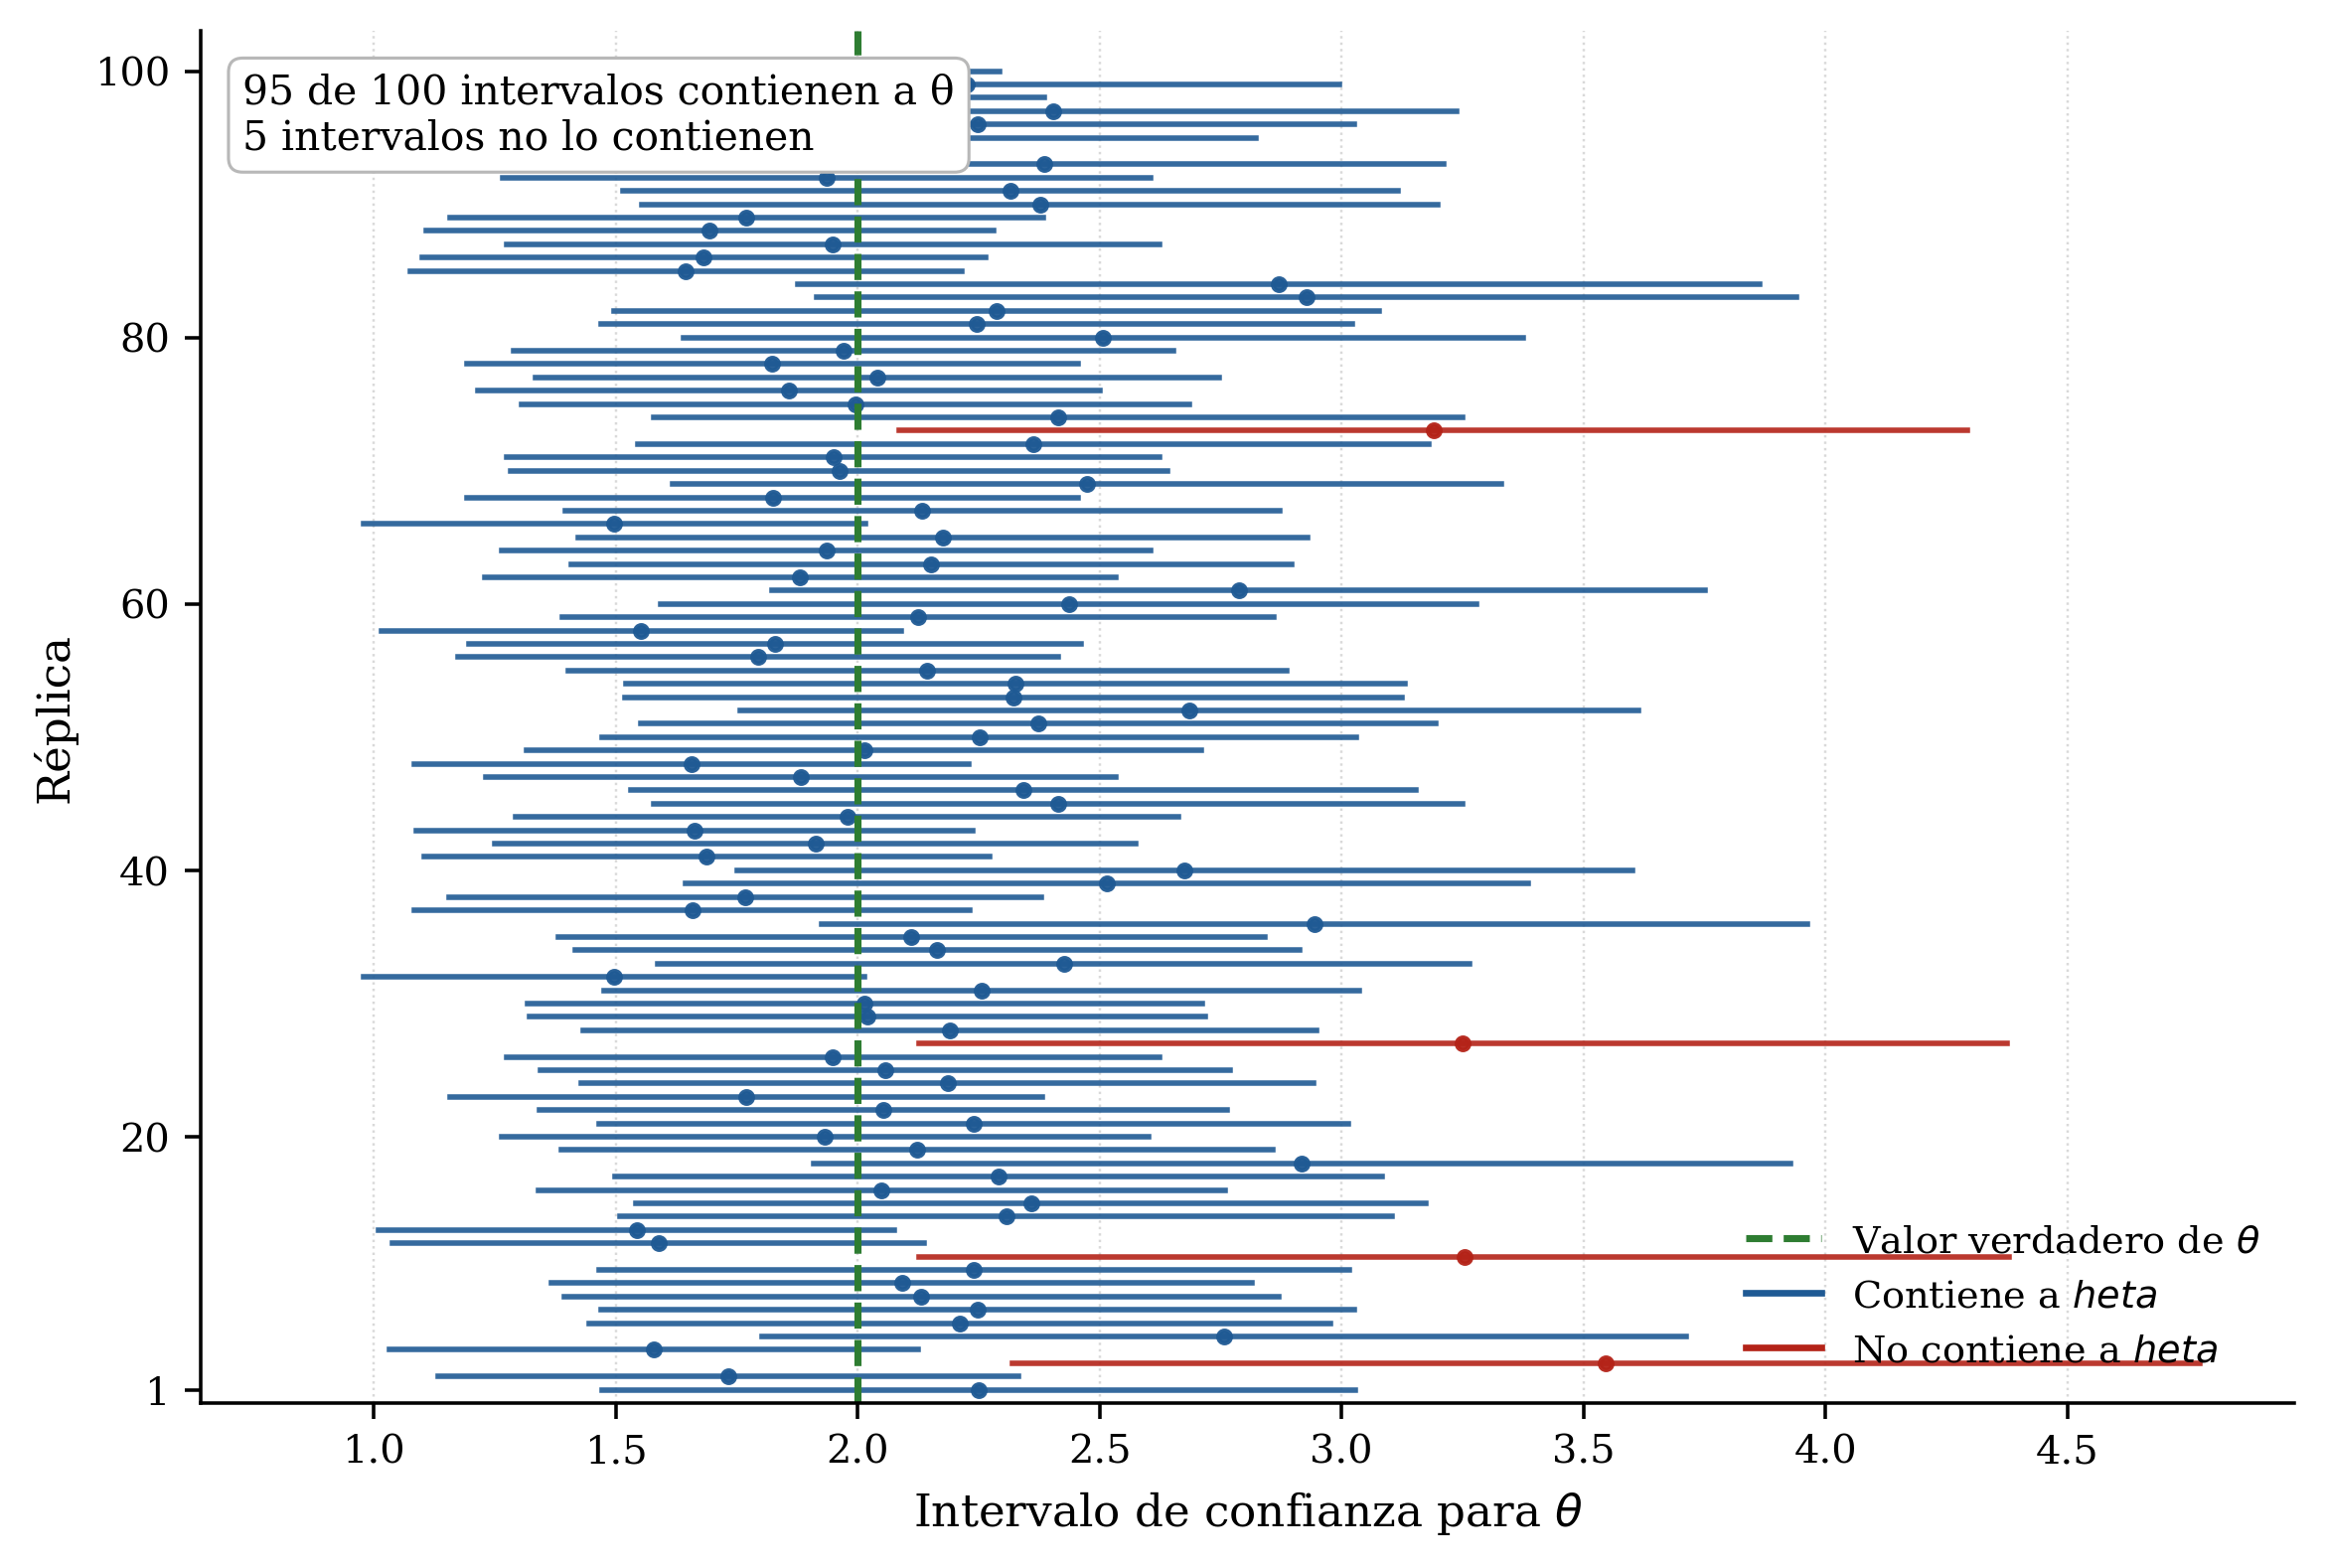
\includegraphics[width=0.91\linewidth]{figures_clear/problema1_intervalos.png}
\caption{Intervalos de confianza exactos para la tasa exponencial. El color distingue los intervalos que contienen el valor verdadero de aquellos que no lo contienen.}
\label{fig:p1}
\end{figure}
\FloatBarrier

\subsection*{Interpretación Figura 1}

Cada segmento horizontal es el resultado de aplicar el mismo método a una muestra diferente. La línea vertical verde indica el valor fijado como verdadero, $\theta=2$. Un intervalo azul atraviesa esa línea y por tanto produce $I_b=1$; un intervalo rojo no la atraviesa y produce $I_b=0$. Con la semilla 1966, 95 de los 100 indicadores valen uno, por lo que
\begin{equation*}
\widehat C_{100}=\frac{95}{100}=0.95.
\end{equation*}
Esta proporción es la cobertura empírica mostrada en la figura. Su coincidencia exacta con $0.95$ es particular de esta ejecución y no debe entenderse como una prueba por sí sola. Si se cambia la semilla, el número de intervalos que cubren puede ser 93, 96 u otro valor cercano. La teoría es la que establece la cobertura exacta; la simulación permite observar cómo se manifiesta en muestras repetidas.

La posición y longitud de los intervalos cambian porque $S_b$ es aleatoria. Si una muestra produce una suma pequeña, los cocientes que forman los extremos son mayores y el intervalo se desplaza hacia la derecha; si la suma es grande, se desplaza hacia la izquierda. Los intervalos rojos representan las fallas esperadas del procedimiento. Un nivel del $95\%$ admite aproximadamente un $5\%$ de fallas cuando el experimento se repite muchas veces.

\section{Problema 2}

\paragraph{Descripción del problema.}
Se debe determinar el tamaño de muestra necesario para estimar la proporción de votantes que apoyan al candidato A con un nivel de confianza del $90\%$ y un margen de error de $0.03$. Además, se revisa mediante el modelo binomial y simulación qué tan precisa es la aproximación utilizada.

\subsection*{Traducción del problema a variables Bernoulli}

Primero se representa la respuesta de cada votante mediante
\begin{equation*}
X_i=
\begin{cases}
1, & \text{si el votante $i$ manifiesta que votará por A},\\
0, & \text{en otro caso}.
\end{cases}
\end{equation*}
Entonces $X_i\sim\operatorname{Bernoulli}(\theta)$, donde $\theta$ es la proporción poblacional de apoyo. La suma
\begin{equation*}
K=\sum_{i=1}^{n}X_i
\end{equation*}
cuenta cuántos entrevistados apoyan al candidato, por lo que
\begin{equation*}
K\sim\operatorname{Binomial}(n,\theta),
\qquad
\overline X=\frac{K}{n}.
\end{equation*}
Esta representación permite usar la aproximación normal y, después, calcular la cobertura con la distribución binomial.

\subsection*{Cálculo usual mediante aproximación normal}

La media muestral tiene
\begin{equation*}
\E[\overline X]=\theta,
\qquad
\Var(\overline X)=\frac{\theta(1-\theta)}{n}.
\end{equation*}
Para $n$ grande, el teorema central del límite permite aproximar
\begin{equation*}
\frac{\overline X-\theta}{\sqrt{\theta(1-\theta)/n}}\approx N(0,1).
\end{equation*}
Un intervalo normal de confianza $1-\alpha$ tiene un margen aproximado
\begin{equation*}
E=z_{1-\alpha/2}\sqrt{\frac{\theta(1-\theta)}{n}}.
\end{equation*}
En este caso $1-\alpha=0.90$, de modo que $z_{0.95}=1.644854$, y se desea $E=0.03$. El inconveniente es que $\theta$ todavía es desconocido. Para escoger un tamaño que funcione sin tener una estimación previa, se usa el mayor valor posible de $\theta(1-\theta)$. Completando el cuadrado,
\begin{equation*}
\theta(1-\theta)=\frac14-\left(\theta-\frac12\right)^2\leq\frac14,
\end{equation*}
con igualdad en $\theta=0.5$. Este es el llamado peor caso, porque produce el error estándar más grande. Por tanto,
\begin{equation*}
1.644854\sqrt{\frac{1}{4n}}\leq0.03,
\end{equation*}
y al despejar $n$,
\begin{equation}
\boxed{
 n\geq\frac{1.644854^2(0.25)}{0.03^2}=751.54
 \quad\Longrightarrow\quad n=752.}
\label{eq:n-prop}
\end{equation}
Se redondea hacia arriba porque un tamaño menor ya no satisface la desigualdad aproximada.

\subsection*{Evaluación de la cobertura con la distribución binomial}

El resultado $n=752$ se obtuvo usando el teorema central del límite, por lo que conviene revisar qué probabilidad produce realmente el intervalo cuando se conserva el modelo exacto de los datos. La cantidad $K$ cuenta el número de votantes que apoyan al candidato A. Como es la suma de $n$ variables Bernoulli independientes, $K\sim\operatorname{Binomial}(n,\theta)$. Esta distribución contiene todas las probabilidades posibles de la proporción muestral $\overline X=K/n$ y permite calcular, sin aproximación normal, la probabilidad de que el intervalo pedido contenga a $\theta$. Esa probabilidad es justamente la cobertura del intervalo para el valor de $\theta$ considerado.

El intervalo pedido contiene a $\theta$ cuando
\begin{equation*}
\overline X-0.03\leq\theta\leq\overline X+0.03.
\end{equation*}
Esto es equivalente a
\begin{equation*}
|\overline X-\theta|\leq0.03.
\end{equation*}
Como $\overline X=K/n$, el evento también puede escribirse
\begin{equation*}
\left|\frac{K}{n}-\theta\right|\leq0.03,
\end{equation*}
que, al despejar $K$, queda
\begin{equation*}
n(\theta-0.03)\leq K\leq n(\theta+0.03).
\end{equation*}
Pero $K$ solo toma valores enteros. Por eso los límites correctos son
\begin{equation*}
k_{\min}(\theta)=\max\!\left\{0,\left\lceil n(\theta-0.03)\right\rceil\right\},
\qquad
k_{\max}(\theta)=\min\!\left\{n,\left\lfloor n(\theta+0.03)\right\rfloor\right\}.
\end{equation*}
La probabilidad exacta de cobertura para un valor fijo de $\theta$ es entonces la suma de las probabilidades binomiales correspondientes:
\begin{equation}
C_n(\theta)=
\sum_{k=k_{\min}(\theta)}^{k_{\max}(\theta)}
\binom{n}{k}\theta^k(1-\theta)^{n-k}.
\label{eq:cob-bin}
\end{equation}
Esta expresión no es un nuevo intervalo. Es una forma exacta de evaluar el intervalo $\overline X\pm0.03$ que pide el enunciado. Al calcular~\eqref{eq:cob-bin} para muchos valores de $\theta$ se puede localizar la peor cobertura. Para $n=752$, el mínimo numérico en una malla fina es cercano al $89.9\%$ alrededor de $\theta=0.5$. En la misma búsqueda, $n=767$ es el primer tamaño cuya cobertura queda por encima del $90\%$ en toda la malla evaluada. Este último resultado es una comprobación numérica, no una consecuencia directa de la fórmula normal.

También se puede considerar una garantía que no dependa del teorema central del límite. La desigualdad de Hoeffding para variables Bernoulli establece
\begin{equation*}
P(|\overline X-\theta|\geq E)\leq2e^{-2nE^2}.
\end{equation*}
Si se exige que la probabilidad de error sea como máximo $0.10$ y se usa $E=0.03$,
\begin{equation*}
2e^{-2n(0.03)^2}\leq0.10
\quad\Longrightarrow\quad
n\geq\frac{\log(20)}{2(0.03)^2}=1664.30.
\end{equation*}
Por tanto, $n=1665$ da una garantía no asintótica, aunque es mucho más conservadora. La comparación muestra tres niveles de respuesta: $752$ por aproximación normal, la evaluación exacta de esa elección mediante la binomial y $1665$ como garantía general de Hoeffding.

\subsection*{Procedimiento de simulación}

La expresión~\eqref{eq:cob-bin} permite calcular la cobertura exacta, pero la simulación es útil para comprobar el cálculo y para mostrar cómo se obtendría la cobertura cuando no fuera posible sumar las probabilidades de forma cerrada. Para un valor fijo de $\theta$, la cobertura buscada es
\begin{equation*}
C_n(\theta)=P_\theta\!\left(\left|\frac{K}{n}-\theta\right|\leq0.03\right).
\end{equation*}
En la réplica $b$ se genera $K_b\sim\operatorname{Binomial}(n,\theta)$ y se define
\begin{equation*}
I_b=\ind\!\left\{\left|\frac{K_b}{n}-\theta\right|\leq0.03\right\}.
\end{equation*}
Se puede generar directamente una binomial porque $K_b$ es exactamente la suma de las $n$ respuestas Bernoulli. Simular $K_b$ o simular uno por uno los $n$ votantes produce el mismo modelo, pero la primera opción es computacionalmente más rápida.

La cobertura empírica para ese valor de $\theta$ es
\begin{equation*}
\widehat C_{n,B}(\theta)=\frac1B\sum_{b=1}^{B}I_b.
\end{equation*}
Nuevamente, $\E[I_b]=C_n(\theta)$, de modo que la ley de los grandes números justifica usar el promedio como aproximación de la cobertura. Su error Monte Carlo puede estimarse mediante
\begin{equation*}
\sqrt{\frac{\widehat C_{n,B}(\theta)[1-\widehat C_{n,B}(\theta)]}{B}}.
\end{equation*}

Como $\theta$ es desconocido y puede tomar cualquier valor entre cero y uno, la evaluación no debe hacerse en un único punto. Se construye una malla, por ejemplo $0.001,0.002,\ldots,0.999$, y para cada valor se calcula la cobertura exacta o su aproximación simulada. El mínimo de la curva representa el caso más desfavorable dentro de la malla. Este procedimiento explica por qué no basta con revisar solamente $\theta=0.5$: aunque allí se maximiza la varianza Bernoulli, la discreción puede hacer que el mínimo exacto aparezca ligeramente desplazado.

En la figura se presenta la cobertura exacta, no una curva Monte Carlo, porque puede obtenerse directamente de~\eqref{eq:cob-bin}. La simulación funciona como verificación independiente: con un número grande de repeticiones, sus puntos deberían quedar próximos a la curva exacta.

Como verificación numérica concreta se tomó $n=752$, $\theta=0.5$, margen $E=0.03$, $B=50\,000$ y semilla 1966. La suma binomial exacta da
\begin{equation*}
C_{752}(0.5)=0.899263,
\end{equation*}
mientras que la simulación produjo
\begin{equation*}
\widehat C_{752,50\,000}(0.5)=0.89876,
\qquad
\operatorname{EMC}\approx0.00135.
\end{equation*}
La diferencia entre $89.9263\%$ y $89.876\%$ es menor que un error Monte Carlo, por lo que el experimento reproduce adecuadamente la probabilidad binomial. Este cálculo muestra el papel de Monte Carlo: no sustituye la suma exacta cuando esta está disponible, sino que la comprueba y proporciona un procedimiento que también puede usarse cuando la cobertura no tiene una expresión cerrada sencilla.

\begin{figure}[!htbp]
\centering
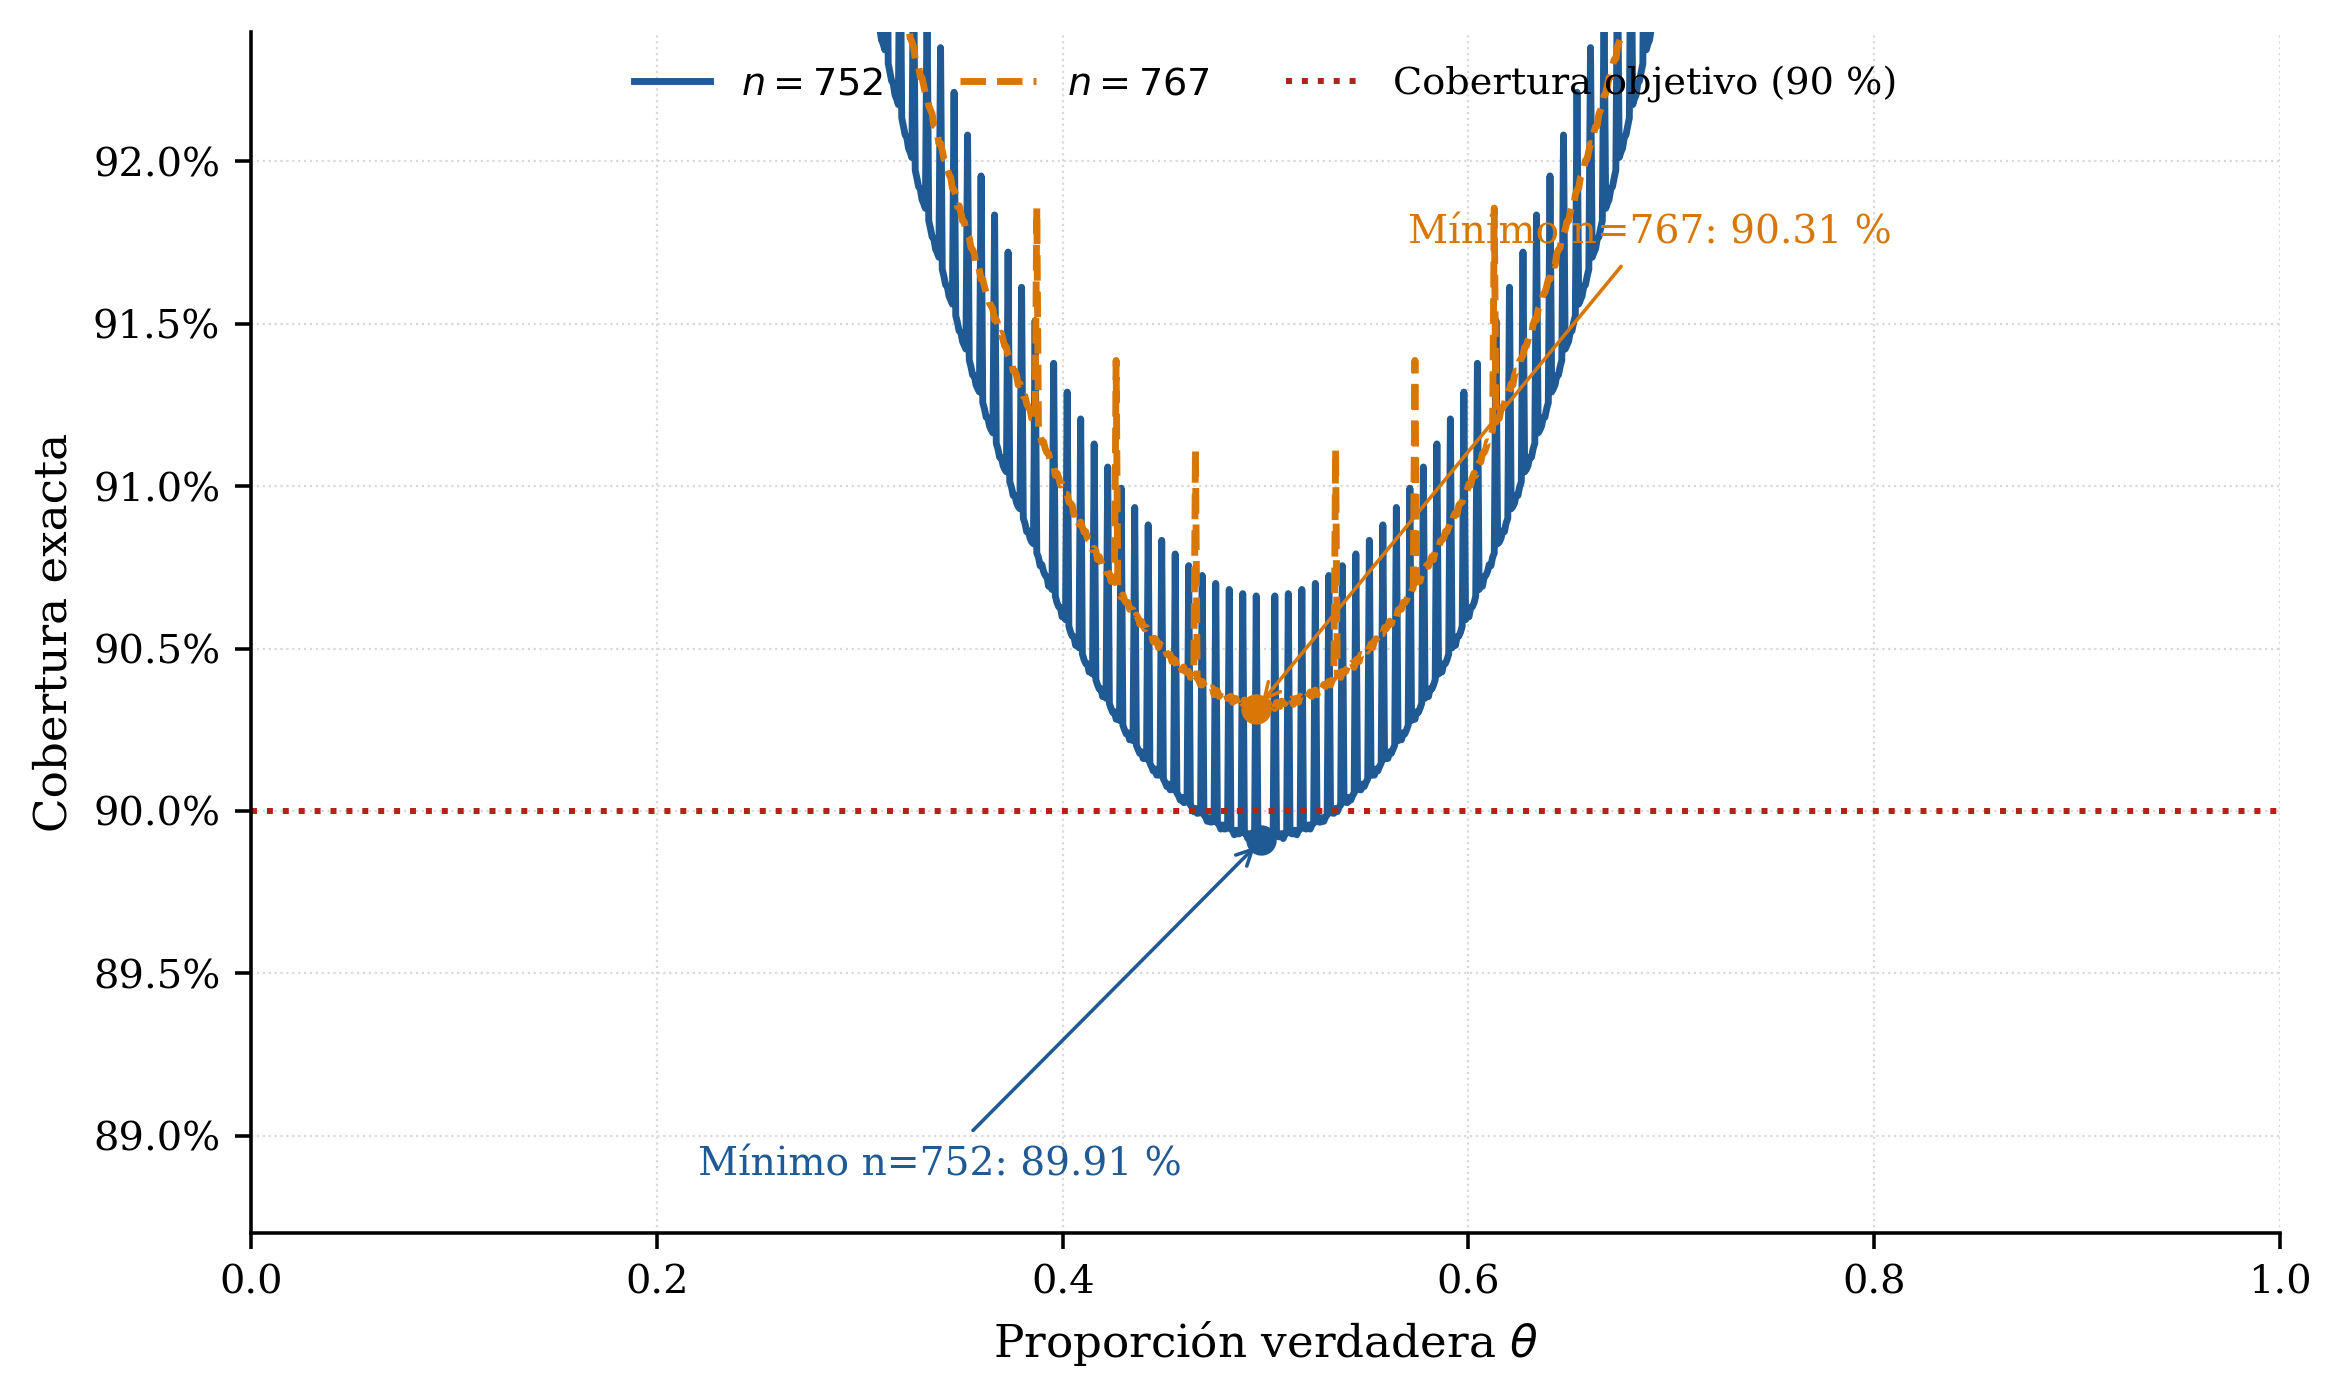
\includegraphics[width=0.91\linewidth]{figures_clear/problema2_cobertura.png}
\caption{Cobertura binomial exacta del intervalo $\overline X\pm0.03$ para dos tamaños de muestra.}
\label{fig:p2}
\end{figure}
\FloatBarrier

\subsection*{Interpretación Figura 2}

El eje horizontal recorre los valores posibles de $\theta$ y el eje vertical muestra la probabilidad exacta de que el intervalo contenga a ese valor. La línea roja horizontal es la cobertura objetivo del $90\%$. La curva azul para $n=752$ oscila alrededor de esa referencia y presenta un mínimo de aproximadamente $89.91\%$. Por tanto, la respuesta normal es muy cercana, pero no garantiza exactamente el $90\%$ para todo $\theta$.

Las oscilaciones aparecen porque la binomial es discreta. Cuando $\theta$ cambia un poco, los límites reales $n(\theta\pm0.03)$ cambian continuamente, pero los enteros admitidos para $K$ solo cambian cuando se cruza un entero; cada cambio modifica de golpe la suma de probabilidades en~\eqref{eq:cob-bin}. Para $n=767$, la curva naranja queda por encima del objetivo en la malla utilizada. La peor situación continúa cerca de $0.5$, donde la varianza Bernoulli es mayor.

\section{Problema 3}

\paragraph{Descripción del problema.}
Primero se debe demostrar una cota superior para la varianza de cualquier variable aleatoria cuyo soporte esté contenido en $[a,b]$. Después, esa cota se utiliza para construir un intervalo de confianza para la media de una distribución desconocida cuando el tamaño de muestra es grande.

\subsection*{Demostración de la cota de varianza}

Se supone que $a\leq X\leq b$ con probabilidad uno. La idea es construir una expresión cuyo signo sea conocido. Como $X-a\geq0$ y $b-X\geq0$,
\begin{equation*}
(X-a)(b-X)\geq0.
\end{equation*}
Al desarrollar,
\begin{equation*}
-X^2+(a+b)X-ab\geq0,
\end{equation*}
por lo que
\begin{equation*}
X^2\leq(a+b)X-ab.
\end{equation*}
Tomando esperanza y escribiendo $\mu=\E[X]$,
\begin{equation*}
\E[X^2]\leq(a+b)\mu-ab.
\end{equation*}
Ahora se usa la identidad $\Var(X)=\E[X^2]-\mu^2$:
\begin{align*}
\Var(X)
&\leq(a+b)\mu-ab-\mu^2\\
&=\frac{(b-a)^2}{4}-\left(\mu-\frac{a+b}{2}\right)^2\\
&\leq\frac{(b-a)^2}{4}.
\end{align*}
En el último paso se usa que un cuadrado siempre es no negativo. Así se concluye
\begin{equation}
\boxed{\Var(X)\leq\frac{(b-a)^2}{4}.}
\label{eq:popoviciu}
\end{equation}
La igualdad requiere que el término cuadrático sea cero, es decir, que $\mu=(a+b)/2$, y que la desigualdad inicial se cumpla con igualdad en promedio. Esto ocurre cuando $X$ concentra probabilidad $1/2$ en $a$ y $1/2$ en $b$.

\subsection*{Intervalo de confianza para la media}

Sea $X_1,\ldots,X_n$ una muestra de una distribución desconocida, pero con soporte en $[a,b]$. Si $n$ es grande, el teorema central del límite sugiere
\begin{equation*}
\frac{\overline X-\mu}{\sigma/\sqrt n}\approx N(0,1),
\qquad \sigma^2=\Var(X).
\end{equation*}
El problema es que $\sigma$ también es desconocida. La cota~\eqref{eq:popoviciu} implica
\begin{equation*}
\sigma\leq\frac{b-a}{2}.
\end{equation*}
Si se reemplaza el error estándar desconocido $\sigma/\sqrt n$ por su máximo posible $(b-a)/(2\sqrt n)$, se obtiene el intervalo conservador
\begin{equation}
\boxed{
\overline X\pm z_{1-\alpha/2}\frac{b-a}{2\sqrt n}.}
\label{eq:ic-acotada}
\end{equation}
Se llama conservador porque se calcula como si la distribución tuviera la mayor varianza permitida por el soporte. Para una distribución con varianza menor, el intervalo será más ancho de lo estrictamente necesario. Como el argumento usa el teorema central del límite, la justificación es asintótica y depende de que $n$ sea grande, tal como indica el enunciado.

Si se desea una garantía sin aproximación normal, la desigualdad de Hoeffding para variables acotadas establece
\begin{equation*}
P(|\overline X-\mu|\geq\varepsilon)
\leq2\exp\!\left(-\frac{2n\varepsilon^2}{(b-a)^2}\right).
\end{equation*}
Al igualar el lado derecho a $\alpha$ y despejar $\varepsilon$,
\begin{equation*}
\varepsilon=(b-a)\sqrt{\frac{\log(2/\alpha)}{2n}},
\end{equation*}
lo que produce
\begin{equation*}
\boxed{
\overline X\pm(b-a)\sqrt{\frac{\log(2/\alpha)}{2n}}.}
\end{equation*}
Este intervalo suele ser más ancho, pero su garantía no depende de la forma de la distribución ni de una aproximación normal.

\subsection*{Procedimiento de simulación}

En este problema hay dos afirmaciones diferentes por estudiar: la cota de la varianza y el desempeño del intervalo para la media. La simulación no reemplaza la demostración de~\eqref{eq:popoviciu}; únicamente ayuda a visualizarla y a revisar el comportamiento de los intervalos en distribuciones concretas.

Para la primera parte se considera la familia más sencilla que puede alcanzar la igualdad: una variable que toma solamente los extremos $a$ y $b$,
\begin{equation*}
P(X=a)=p,
\qquad
P(X=b)=1-p.
\end{equation*}
Su media es $pa+(1-p)b$ y, al calcular la varianza, se obtiene
\begin{equation*}
\Var(X)=p(1-p)(b-a)^2.
\end{equation*}
Se evalúa esta expresión para valores de $p$ entre cero y uno. También podría generarse una muestra grande para cada $p$ y calcular la varianza muestral; esta se acercaría a la curva teórica. Se usa esta familia porque la demostración mostró que el máximo solo puede alcanzarse cuando la masa se concentra en los extremos y la media queda en el punto medio.

Para la segunda parte se fija una distribución soportada en $[a,b]$, un tamaño $n$ y un nivel $1-\alpha$. En cada réplica se generan $X_{1,b},\ldots,X_{n,b}$, se calcula $\overline X_b$ y se construyen dos intervalos:
\begin{align*}
I^{(N)}_b&=\left[\overline X_b-z_{1-\alpha/2}\frac{b-a}{2\sqrt n},
\overline X_b+z_{1-\alpha/2}\frac{b-a}{2\sqrt n}\right],\\
I^{(H)}_b&=\left[\overline X_b-(b-a)\sqrt{\frac{\log(2/\alpha)}{2n}},
\overline X_b+(b-a)\sqrt{\frac{\log(2/\alpha)}{2n}}\right].
\end{align*}
Para cada método se registra si el intervalo contiene la media verdadera $\mu$ y se calcula la proporción de coberturas. También se registra la longitud $U_b-L_b$, porque dos métodos pueden tener coberturas parecidas pero precisiones distintas.

Conviene repetir el experimento con distribuciones de formas diferentes: una uniforme, una beta reescalada concentrada en el centro y la distribución de dos puntos en los extremos. Esta última representa el caso más exigente porque alcanza la varianza máxima. Si el intervalo conservador funciona adecuadamente allí, se espera que sea aún más holgado para distribuciones con menor varianza. La comparación entre cobertura y longitud permite entender el costo de la protección adicional: Hoeffding ofrece una garantía más general, pero normalmente produce intervalos más largos.

\begin{figure}[!htbp]
\centering
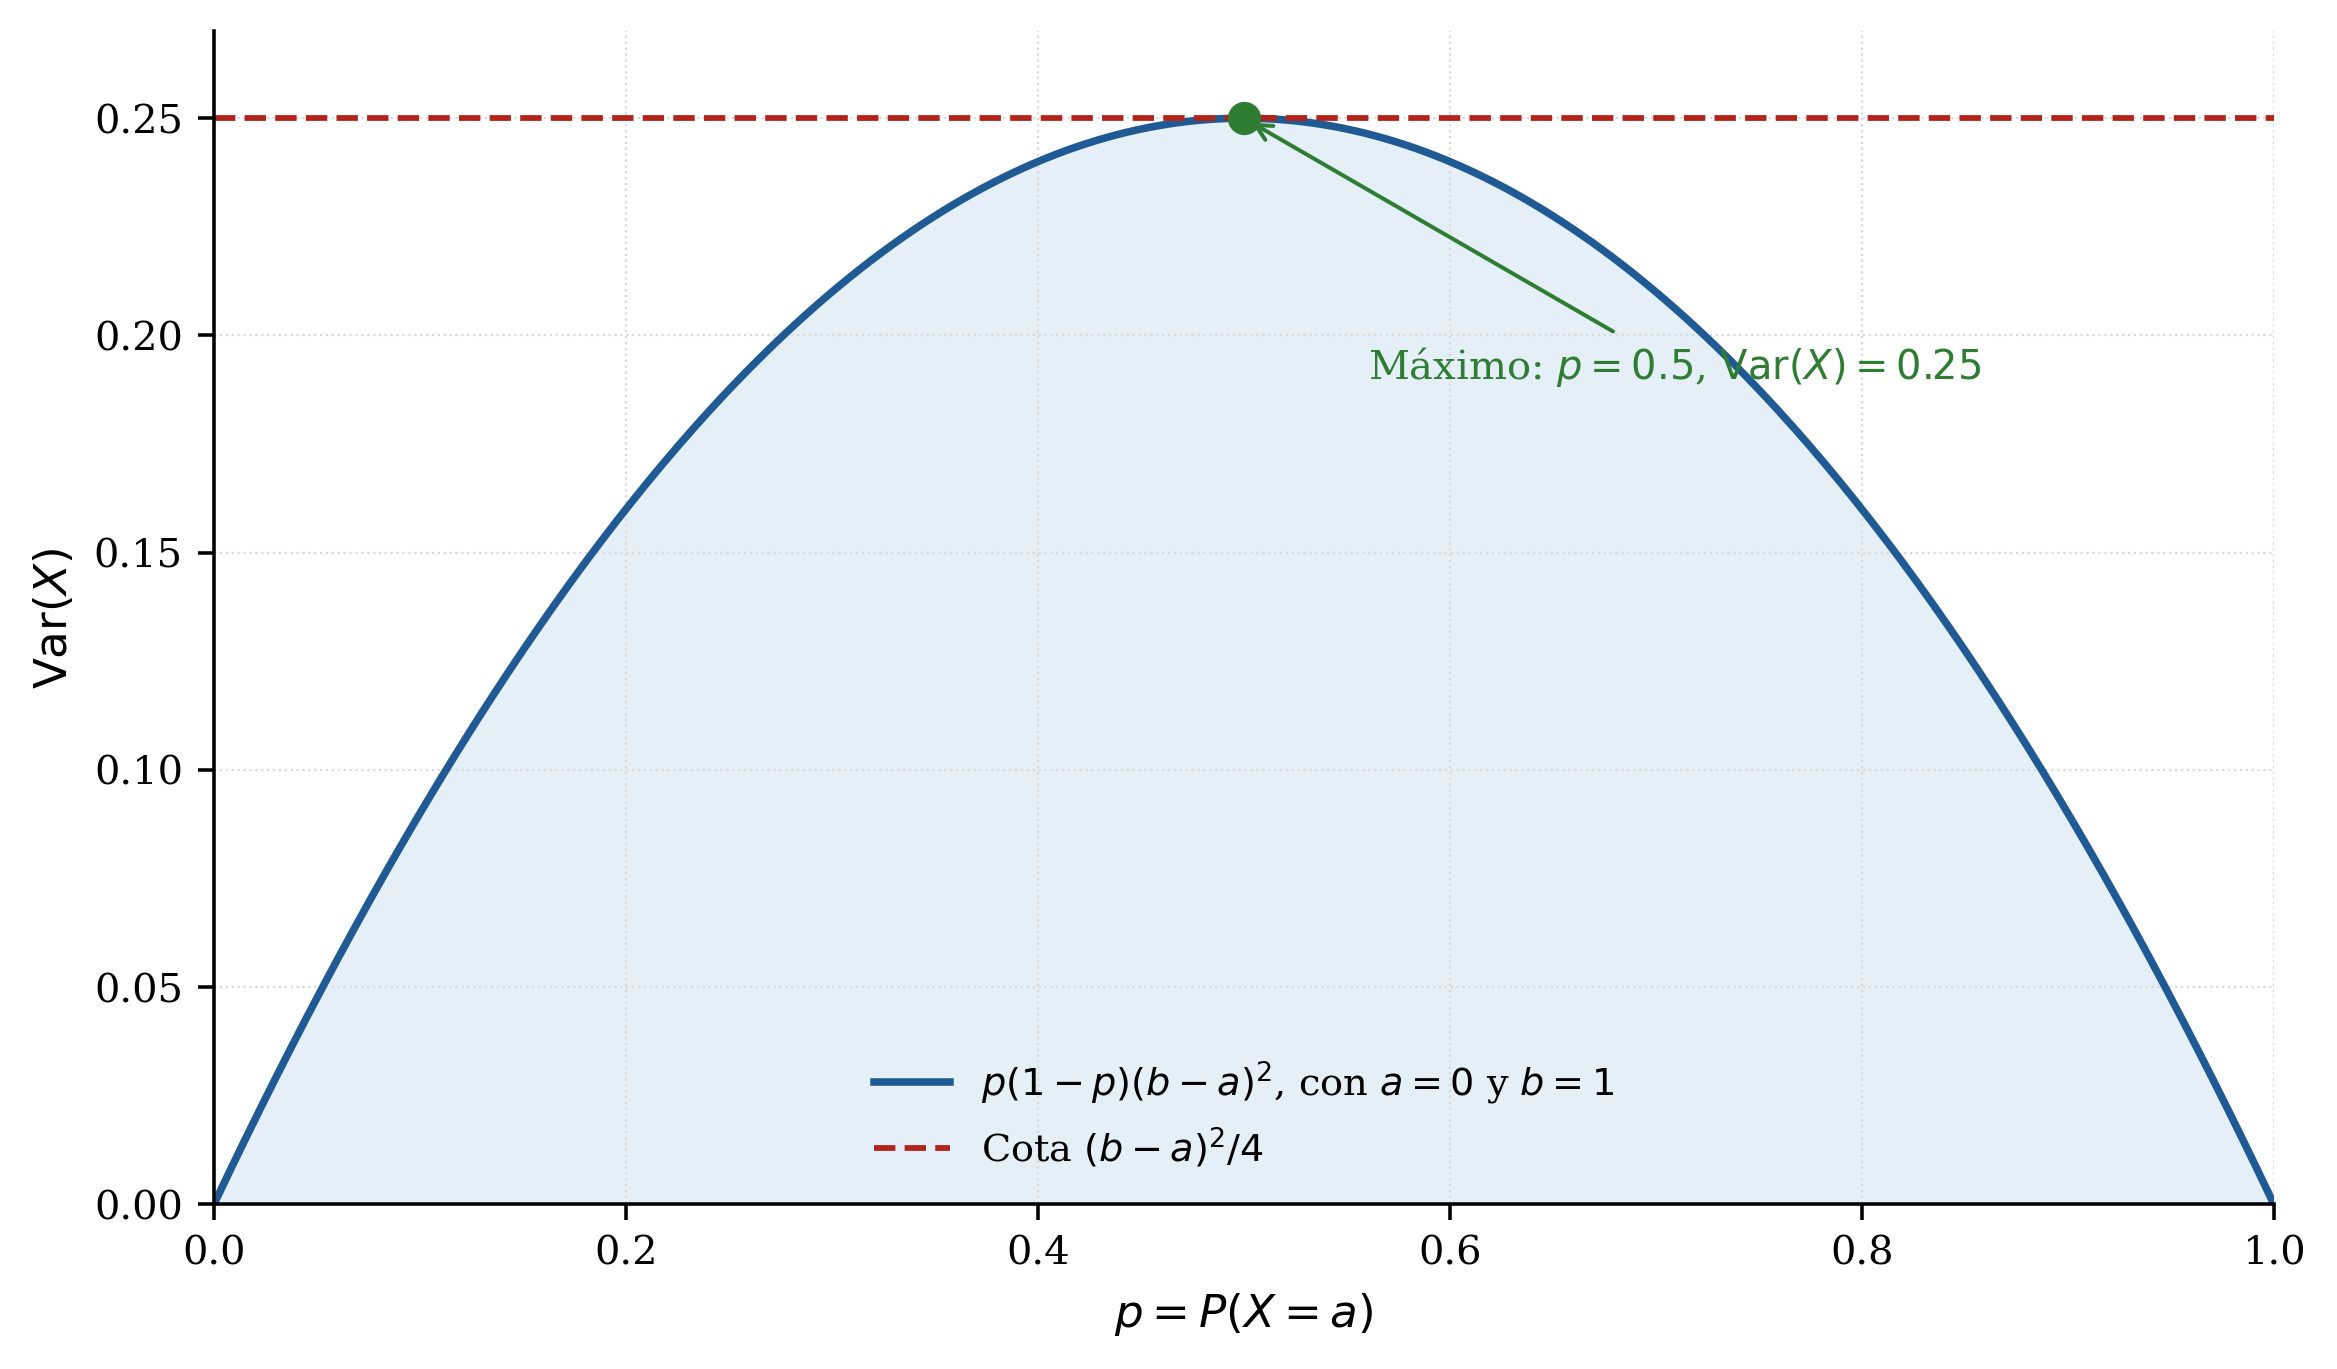
\includegraphics[width=0.90\linewidth]{figures_clear/problema3_varianza.png}
\caption{Varianza de una distribución de dos puntos y cota máxima para variables en $[0,1]$.}
\label{fig:p3}
\end{figure}
\FloatBarrier

\subsection*{Interpretación Figura 3}

La figura toma $a=0$ y $b=1$. Para cada valor de $p$ se considera una variable que vale cero con probabilidad $p$ y uno con probabilidad $1-p$. El eje horizontal representa esa probabilidad y el eje vertical la varianza teórica $p(1-p)$. Cuando $p=0$ o $p=1$, la variable siempre toma un único valor y su varianza es cero. Al repartir la probabilidad entre los dos extremos, la dispersión aumenta.

El máximo aparece en $p=0.5$, donde la masa queda dividida por igual y la varianza vale $0.25$. El punto verde coincide con la línea roja correspondiente a $(b-a)^2/4=1/4$. La figura confirma visualmente el caso de igualdad identificado en la demostración. No constituye por sí sola una prueba para todas las distribuciones; esa garantía proviene del desarrollo algebraico anterior.

Esta misma configuración explica por qué el intervalo conservador usa $(b-a)/(2\sqrt n)$ como error estándar máximo. La distribución de dos puntos es el escenario de mayor variabilidad permitido por el soporte. Para distribuciones más concentradas, el verdadero error estándar es menor y el intervalo será más amplio de lo necesario. En una simulación de cobertura, esto se reflejaría en coberturas iguales o superiores al nivel nominal, acompañadas de una longitud mayor que la de un intervalo que utilizara la varianza real.

\subsection*{Segunda simulación: cobertura y longitud de los intervalos}

Para completar la parte inferencial del problema se realizó un segundo experimento con $a=0$, $b=1$, $n=100$, confianza nominal del $95\%$, $B=50\,000$ y semilla base 1966. Se estudiaron tres distribuciones con media $\mu=0.5$: la distribución de dos puntos con igual masa en 0 y 1, la uniforme en $[0,1]$ y una $\operatorname{Beta}(4,4)$ reescalada. Para cada muestra se construyó el intervalo conservador basado en el teorema central del límite y el intervalo de Hoeffding, y se registró si contenían a $\mu$.

\begin{figure}[!htbp]
\centering
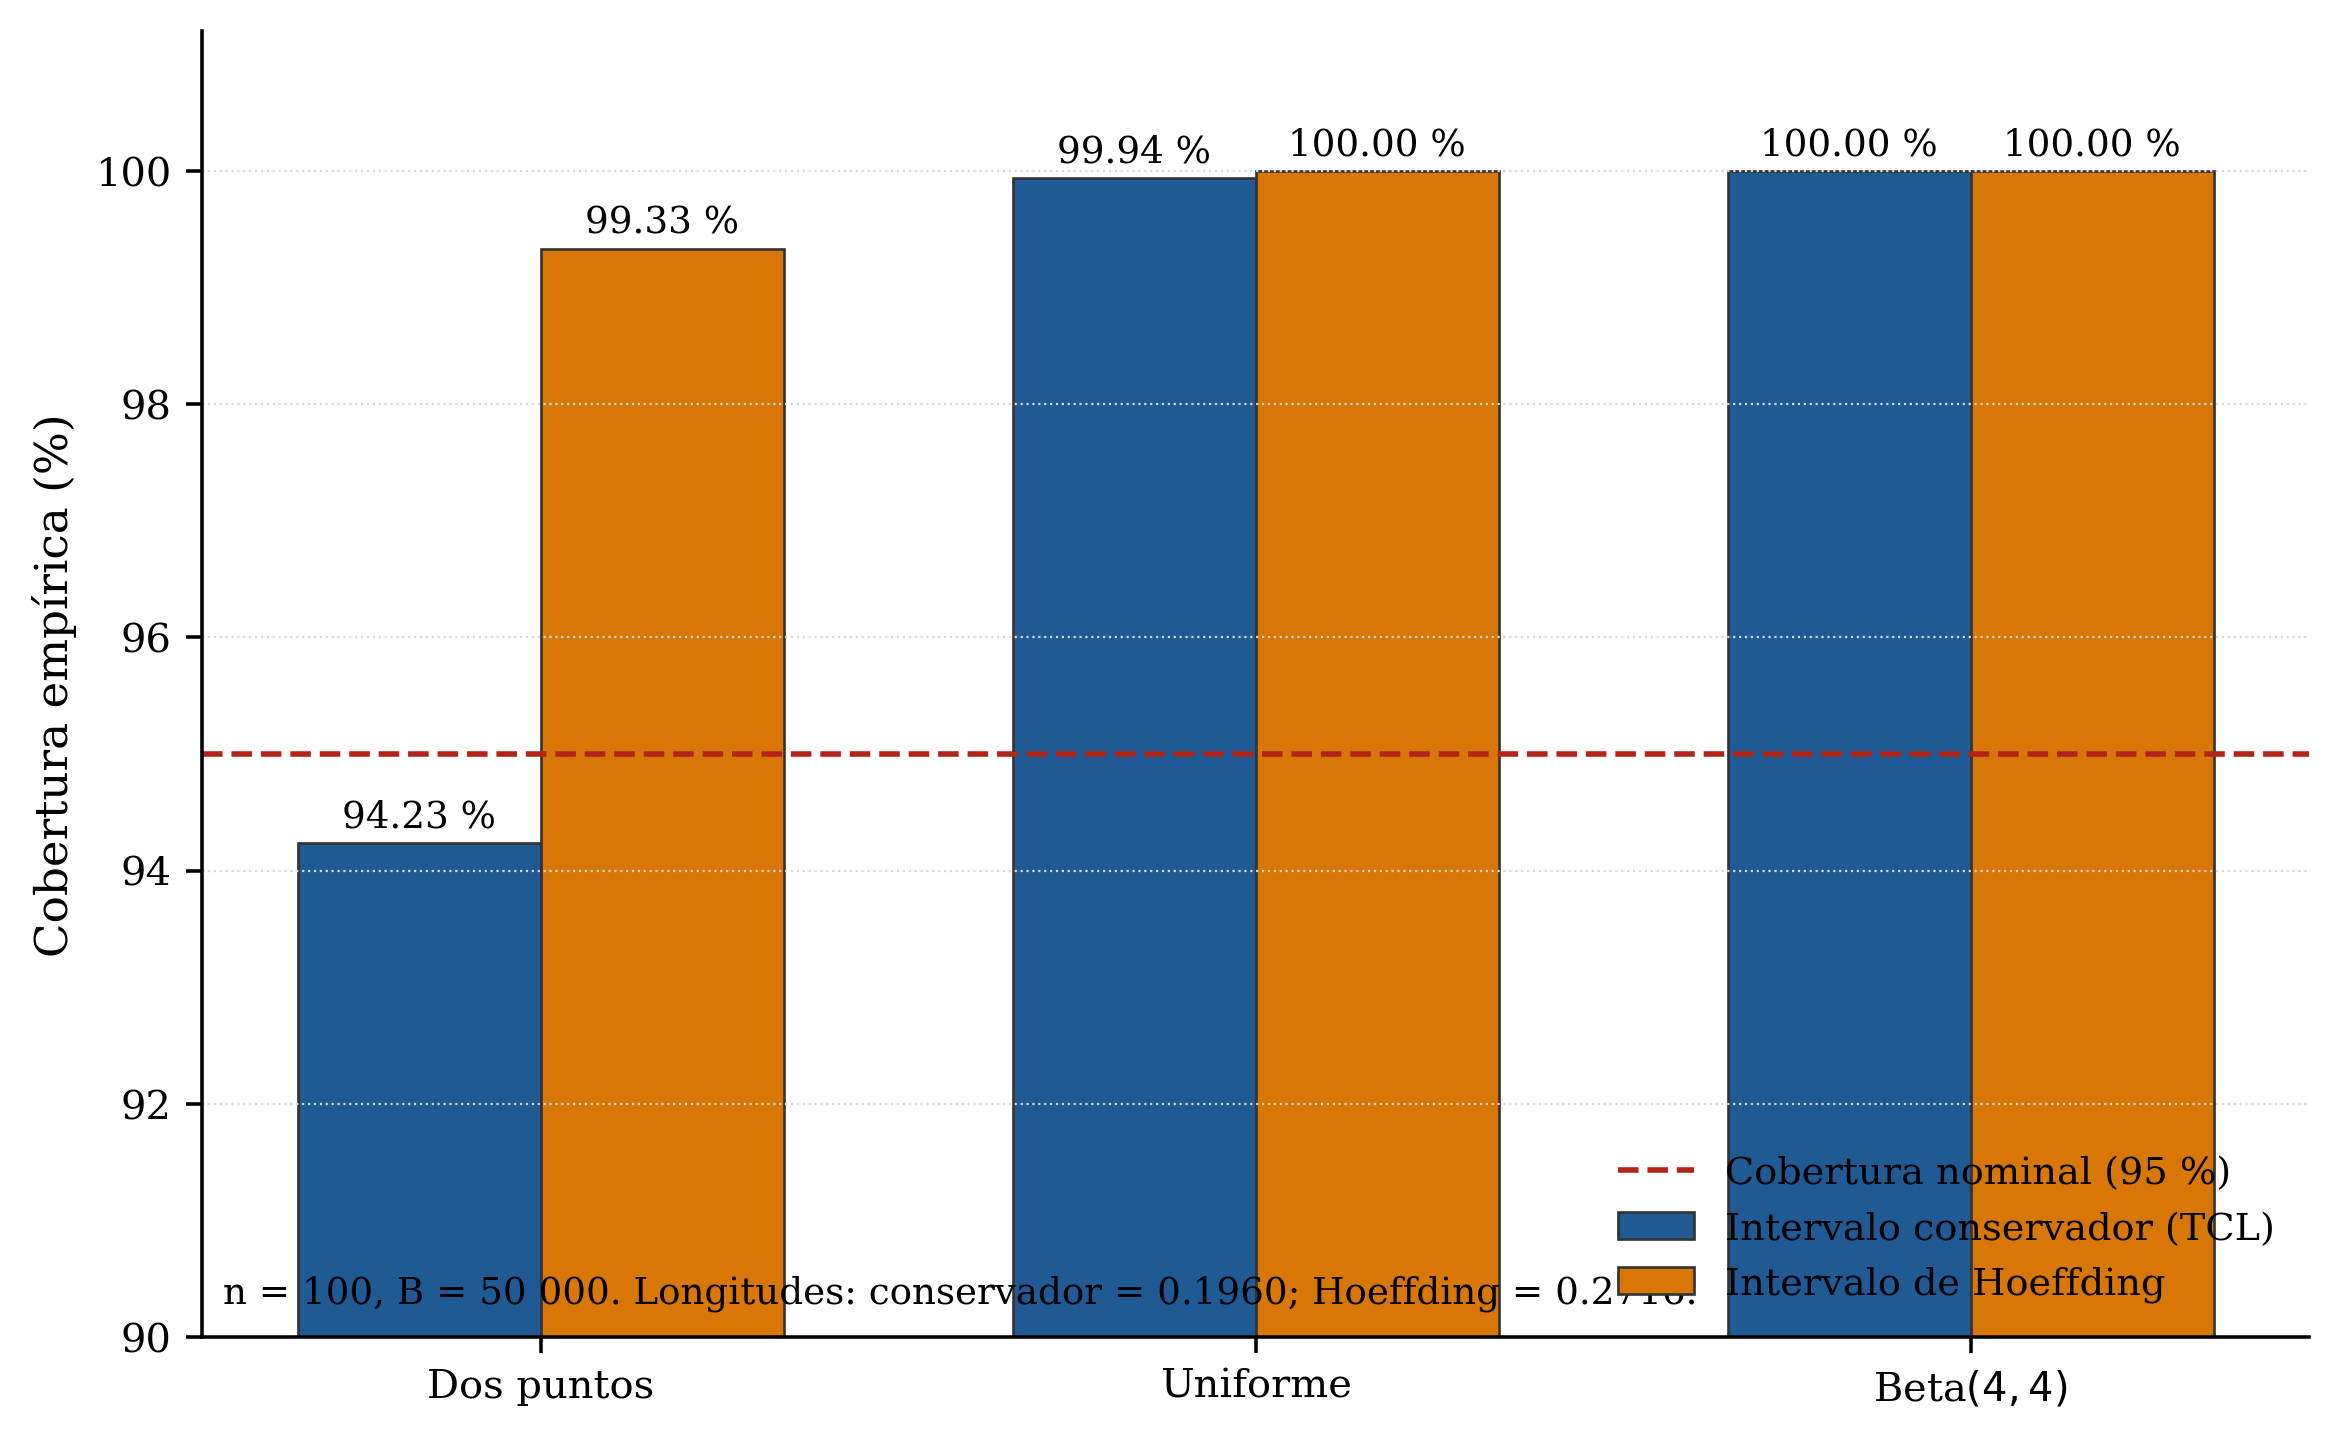
\includegraphics[width=0.91\linewidth]{figures_clear/problema3_cobertura_intervalos.png}
\caption{Cobertura empírica de los intervalos conservador y de Hoeffding para tres distribuciones soportadas en $[0,1]$.}
\label{fig:p3b}
\end{figure}
\FloatBarrier

\subsection*{Interpretación Figura 4}

La distribución de dos puntos es el caso más exigente porque alcanza la varianza máxima $1/4$. Allí el intervalo conservador obtuvo una cobertura de $94.23\%$, cercana al $95\%$ nominal; la diferencia se explica por el carácter asintótico del teorema central del límite y por la variación Monte Carlo. Para la uniforme y la $\operatorname{Beta}(4,4)$, cuyas varianzas son menores, la cobertura aumentó a $99.94\%$ y $100\%$. Esto confirma que usar la varianza máxima protege frente al peor caso, pero puede producir sobrecobertura cuando la distribución está más concentrada.

El intervalo de Hoeffding alcanzó coberturas de $99.33\%$, $100\%$ y $100\%$, respectivamente. Su comportamiento es más conservador porque su garantía no depende de una aproximación normal. Esa protección adicional se paga con una mayor longitud: en esta configuración, la longitud del intervalo conservador es $0.1960$, mientras que la de Hoeffding es $0.2716$. Por tanto, la segunda simulación permite comparar dos aspectos que deben revisarse conjuntamente: la cobertura y la precisión. Un intervalo con cobertura muy alta no necesariamente es preferible si resulta considerablemente más ancho.

\section{Problema 4}

\paragraph{Descripción del problema.}
Se deben obtener los estimadores de $\theta$ por el método de momentos y por máxima verosimilitud para la densidad dada. Luego se estudian su sesgo, consistencia y eficiencia, y se comparan sus resultados mediante una simulación Monte Carlo.

\subsection*{Estimador por método de momentos}

La densidad es
\begin{equation*}
f(x;\theta)=(\theta+1)x^\theta,
\qquad0\leq x\leq1,
\qquad\theta>-1.
\end{equation*}
El método de momentos consiste en igualar un momento teórico con su versión muestral. Como solo hay un parámetro, basta usar el primer momento:
\begin{align*}
\E[X]
&=\int_0^1x(\theta+1)x^\theta\,dx\\
&=(\theta+1)\int_0^1x^{\theta+1}\,dx\\
&=\frac{\theta+1}{\theta+2}.
\end{align*}
Se iguala esta expresión con $\overline X$:
\begin{equation*}
\overline X=\frac{\theta+1}{\theta+2}.
\end{equation*}
Despejando paso a paso,
\begin{equation*}
\overline X(\theta+2)=\theta+1,
\qquad
\theta(\overline X-1)=1-2\overline X,
\end{equation*}
por lo que
\begin{equation}
\boxed{
\widehat\theta_{MM}=\frac{2\overline X-1}{1-\overline X}.}
\label{eq:mm}
\end{equation}

\subsection*{Estimador de máxima verosimilitud}

Para una muestra independiente, la verosimilitud es el producto de las densidades:
\begin{equation*}
L(\theta)
=\prod_{i=1}^{n}(\theta+1)X_i^\theta
=(\theta+1)^n\left(\prod_{i=1}^{n}X_i\right)^\theta.
\end{equation*}
Es más sencillo trabajar con el logaritmo, porque transforma productos en sumas:
\begin{equation*}
\ell(\theta)=n\log(\theta+1)+\theta\sum_{i=1}^{n}\log X_i.
\end{equation*}
La derivada es
\begin{equation*}
\ell'(\theta)=\frac{n}{\theta+1}+\sum_{i=1}^{n}\log X_i.
\end{equation*}
Al igualarla a cero y despejar,
\begin{equation}
\boxed{
\widehat\theta_{EMV}=-\frac{n}{\sum_{i=1}^{n}\log X_i}-1.}
\label{eq:emv}
\end{equation}
Como $0<X_i\leq1$, se tiene $\log X_i\leq0$, así que la expresión es coherente con el espacio $\theta>-1$. Además,
\begin{equation*}
\ell''(\theta)=-\frac{n}{(\theta+1)^2}<0,
\end{equation*}
lo que confirma que el punto crítico es un máximo.

\subsection*{Sesgo de los estimadores}

Para el EMV conviene transformar los datos. Si $Y_i=-\log X_i$, entonces para $y\geq0$,
\begin{align*}
P(Y_i\leq y)
&=P(-\log X_i\leq y)\\
&=P(X_i\geq e^{-y})\\
&=1-F_X(e^{-y}).
\end{align*}
La función de distribución de $X$ es
\begin{equation*}
F_X(x)=\int_0^x(\theta+1)t^\theta\,dt=x^{\theta+1},
\end{equation*}
por lo que
\begin{equation*}
P(Y_i\leq y)=1-e^{-(\theta+1)y}.
\end{equation*}
Así, $Y_i\sim\operatorname{Exp}(\theta+1)$. Si
\begin{equation*}
T=\sum_{i=1}^{n}Y_i=-\sum_{i=1}^{n}\log X_i,
\end{equation*}
entonces $T\sim\operatorname{Gamma}(n,\text{tasa }\theta+1)$ y
\begin{equation*}
\widehat\theta_{EMV}=\frac{n}{T}-1.
\end{equation*}
Para una gamma con forma $n>1$ y tasa $\theta+1$,
\begin{equation*}
\E\!\left[\frac1T\right]=\frac{\theta+1}{n-1}.
\end{equation*}
Por tanto,
\begin{equation*}
\E[\widehat\theta_{EMV}]
=\frac{n(\theta+1)}{n-1}-1
=\theta+\frac{\theta+1}{n-1}.
\end{equation*}
El sesgo es positivo y disminuye a medida que $n$ crece. Si se reemplaza $n$ por $n-1$ en el numerador se obtiene
\begin{equation}
\boxed{
\widetilde\theta=-\frac{n-1}{\sum_{i=1}^{n}\log X_i}-1,}
\label{eq:emv-corrected}
\end{equation}
que es exactamente insesgado para $n>1$.

Para el estimador de momentos, puede escribirse $\widehat\theta_{MM}=g(\overline X)$, con
\begin{equation*}
g(x)=\frac{2x-1}{1-x}.
\end{equation*}
La función es convexa porque $g''(x)=2/(1-x)^3>0$ en $(0,1)$. La desigualdad de Jensen indica que, cuando la esperanza existe,
\begin{equation*}
\E[g(\overline X)]\geq g(\E[\overline X])=\theta,
\end{equation*}
con desigualdad estricta para una muestra no degenerada. Esto permite concluir que el estimador de momentos también tiene sesgo positivo.

\subsection*{Consistencia y comparación de eficiencia}

Por la ley de los grandes números,
\begin{equation*}
\overline X\xrightarrow{p}\E[X]=\frac{\theta+1}{\theta+2}.
\end{equation*}
Como $g$ es continua en ese punto,
\begin{equation*}
\widehat\theta_{MM}=g(\overline X)\xrightarrow{p}\theta.
\end{equation*}
De forma similar, $T/n$ converge en probabilidad a $1/(\theta+1)$, por lo que $n/T-1$ converge a $\theta$. Los dos estimadores son consistentes.

Para comparar su precisión cuando $n$ es grande, se estudian sus varianzas asintóticas. Primero,
\begin{equation*}
\E[X^2]=\frac{\theta+1}{\theta+3},
\end{equation*}
y por tanto
\begin{equation*}
\Var(X)=
\frac{\theta+1}{(\theta+2)^2(\theta+3)}.
\end{equation*}
El método delta usa la aproximación
\begin{equation*}
\Var(g(\overline X))\approx[g'(\E[X])]^2\Var(\overline X).
\end{equation*}
Como $g'(x)=1/(1-x)^2$ y $1-\E[X]=1/(\theta+2)$,
\begin{equation*}
\Avar(\widehat\theta_{MM})
=\frac{(\theta+1)(\theta+2)^2}{n(\theta+3)}.
\end{equation*}
Para el EMV, la segunda derivada de la log-verosimilitud por observación es $-1/(\theta+1)^2$, así que la información de Fisher es
\begin{equation*}
I_1(\theta)=\frac{1}{(\theta+1)^2}.
\end{equation*}
La varianza asintótica del EMV es el inverso de $nI_1(\theta)$:
\begin{equation*}
\Avar(\widehat\theta_{EMV})=\frac{(\theta+1)^2}{n}.
\end{equation*}
Al restar,
\begin{equation*}
\Avar(\widehat\theta_{MM})-\Avar(\widehat\theta_{EMV})
=\frac{\theta+1}{n(\theta+3)}>0.
\end{equation*}
Por ello, el EMV es asintóticamente más eficiente.

\subsection*{Procedimiento de simulación}

La simulación debe reproducir correctamente la distribución propuesta. Como su función de distribución es $F_X(x)=x^{\theta+1}$, se utiliza la transformada inversa. Si $U\sim U(0,1)$, entonces
\begin{equation*}
X=F_X^{-1}(U)=U^{1/(\theta+1)}
\end{equation*}
tiene la densidad requerida. Esta transformación se obtiene resolviendo $u=x^{\theta+1}$ para $x$ y evita depender de una función especializada del programa.

Para un valor verdadero de $\theta$ y un tamaño $n$, se realizan $B$ réplicas. En cada una se generan $n$ observaciones, se calcula $\widehat\theta_{MM}$, $\widehat\theta_{EMV}$ y $\widetilde\theta$, y se guardan los tres resultados. A partir de las $B$ estimaciones de un método se calculan:
\begin{align*}
\overline{\widehat\theta}
&=\frac1B\sum_{b=1}^{B}\widehat\theta_b,\\
\widehat{\operatorname{Sesgo}}
&=\overline{\widehat\theta}-\theta,\\
\widehat{\Var}(\widehat\theta)
&=\frac{1}{B-1}\sum_{b=1}^{B}
(\widehat\theta_b-\overline{\widehat\theta})^2,\\
\widehat{\operatorname{ECM}}
&=\frac1B\sum_{b=1}^{B}(\widehat\theta_b-\theta)^2.
\end{align*}
Estas cantidades son versiones Monte Carlo de las propiedades teóricas. La media de las estimaciones permite revisar el sesgo; la dispersión alrededor de esa media estima la varianza; y el ECM combina ambas fuentes de error. Numéricamente debe cumplirse aproximadamente
\begin{equation*}
\widehat{\operatorname{ECM}}
\approx
\widehat{\Var}(\widehat\theta)
+\widehat{\operatorname{Sesgo}}^{2}.
\end{equation*}

Para estudiar consistencia no basta con una sola elección de $n$. Se repite el experimento para tamaños crecientes. Un estimador consistente debe mostrar una distribución cada vez más concentrada alrededor de $\theta$, lo que se refleja en sesgo y ECM decrecientes. Para estudiar eficiencia se comparan estimadores usando el mismo $n$ y las mismas réplicas: a igualdad de información, el que presente menor varianza o menor ECM es más preciso. La eficiencia asintótica obtenida analíticamente se refiere al comportamiento cuando $n$ es grande; la simulación también permite observar que, con muestras pequeñas, la corrección del sesgo puede cambiar el orden de los ECM.

Como control adicional se fijó $\theta=2$, $n=30$ y $B=50\,000$. Los resultados fueron:
\begin{center}
\begin{tabular}{lrrr}
\toprule
Estimador & Sesgo empírico & Varianza empírica & ECM empírico \\
\midrule
Momentos & 0.0845 & 0.3672 & 0.3743 \\
EMV & 0.1041 & 0.3498 & 0.3606 \\
EMV corregido & 0.0007 & 0.3269 & 0.3269 \\
\bottomrule
\end{tabular}
\end{center}
La identidad $\operatorname{ECM}=\Var+\operatorname{Sesgo}^2$ se cumple numéricamente salvo por redondeo. Esta tabla documenta qué se calcula en una configuración fija, mientras que la Figura~\ref{fig:p4} repite el análisis para tamaños de muestra crecientes con 25\,000 réplicas por valor de $n$ y semilla 1966.

\begin{figure}[!htbp]
\centering
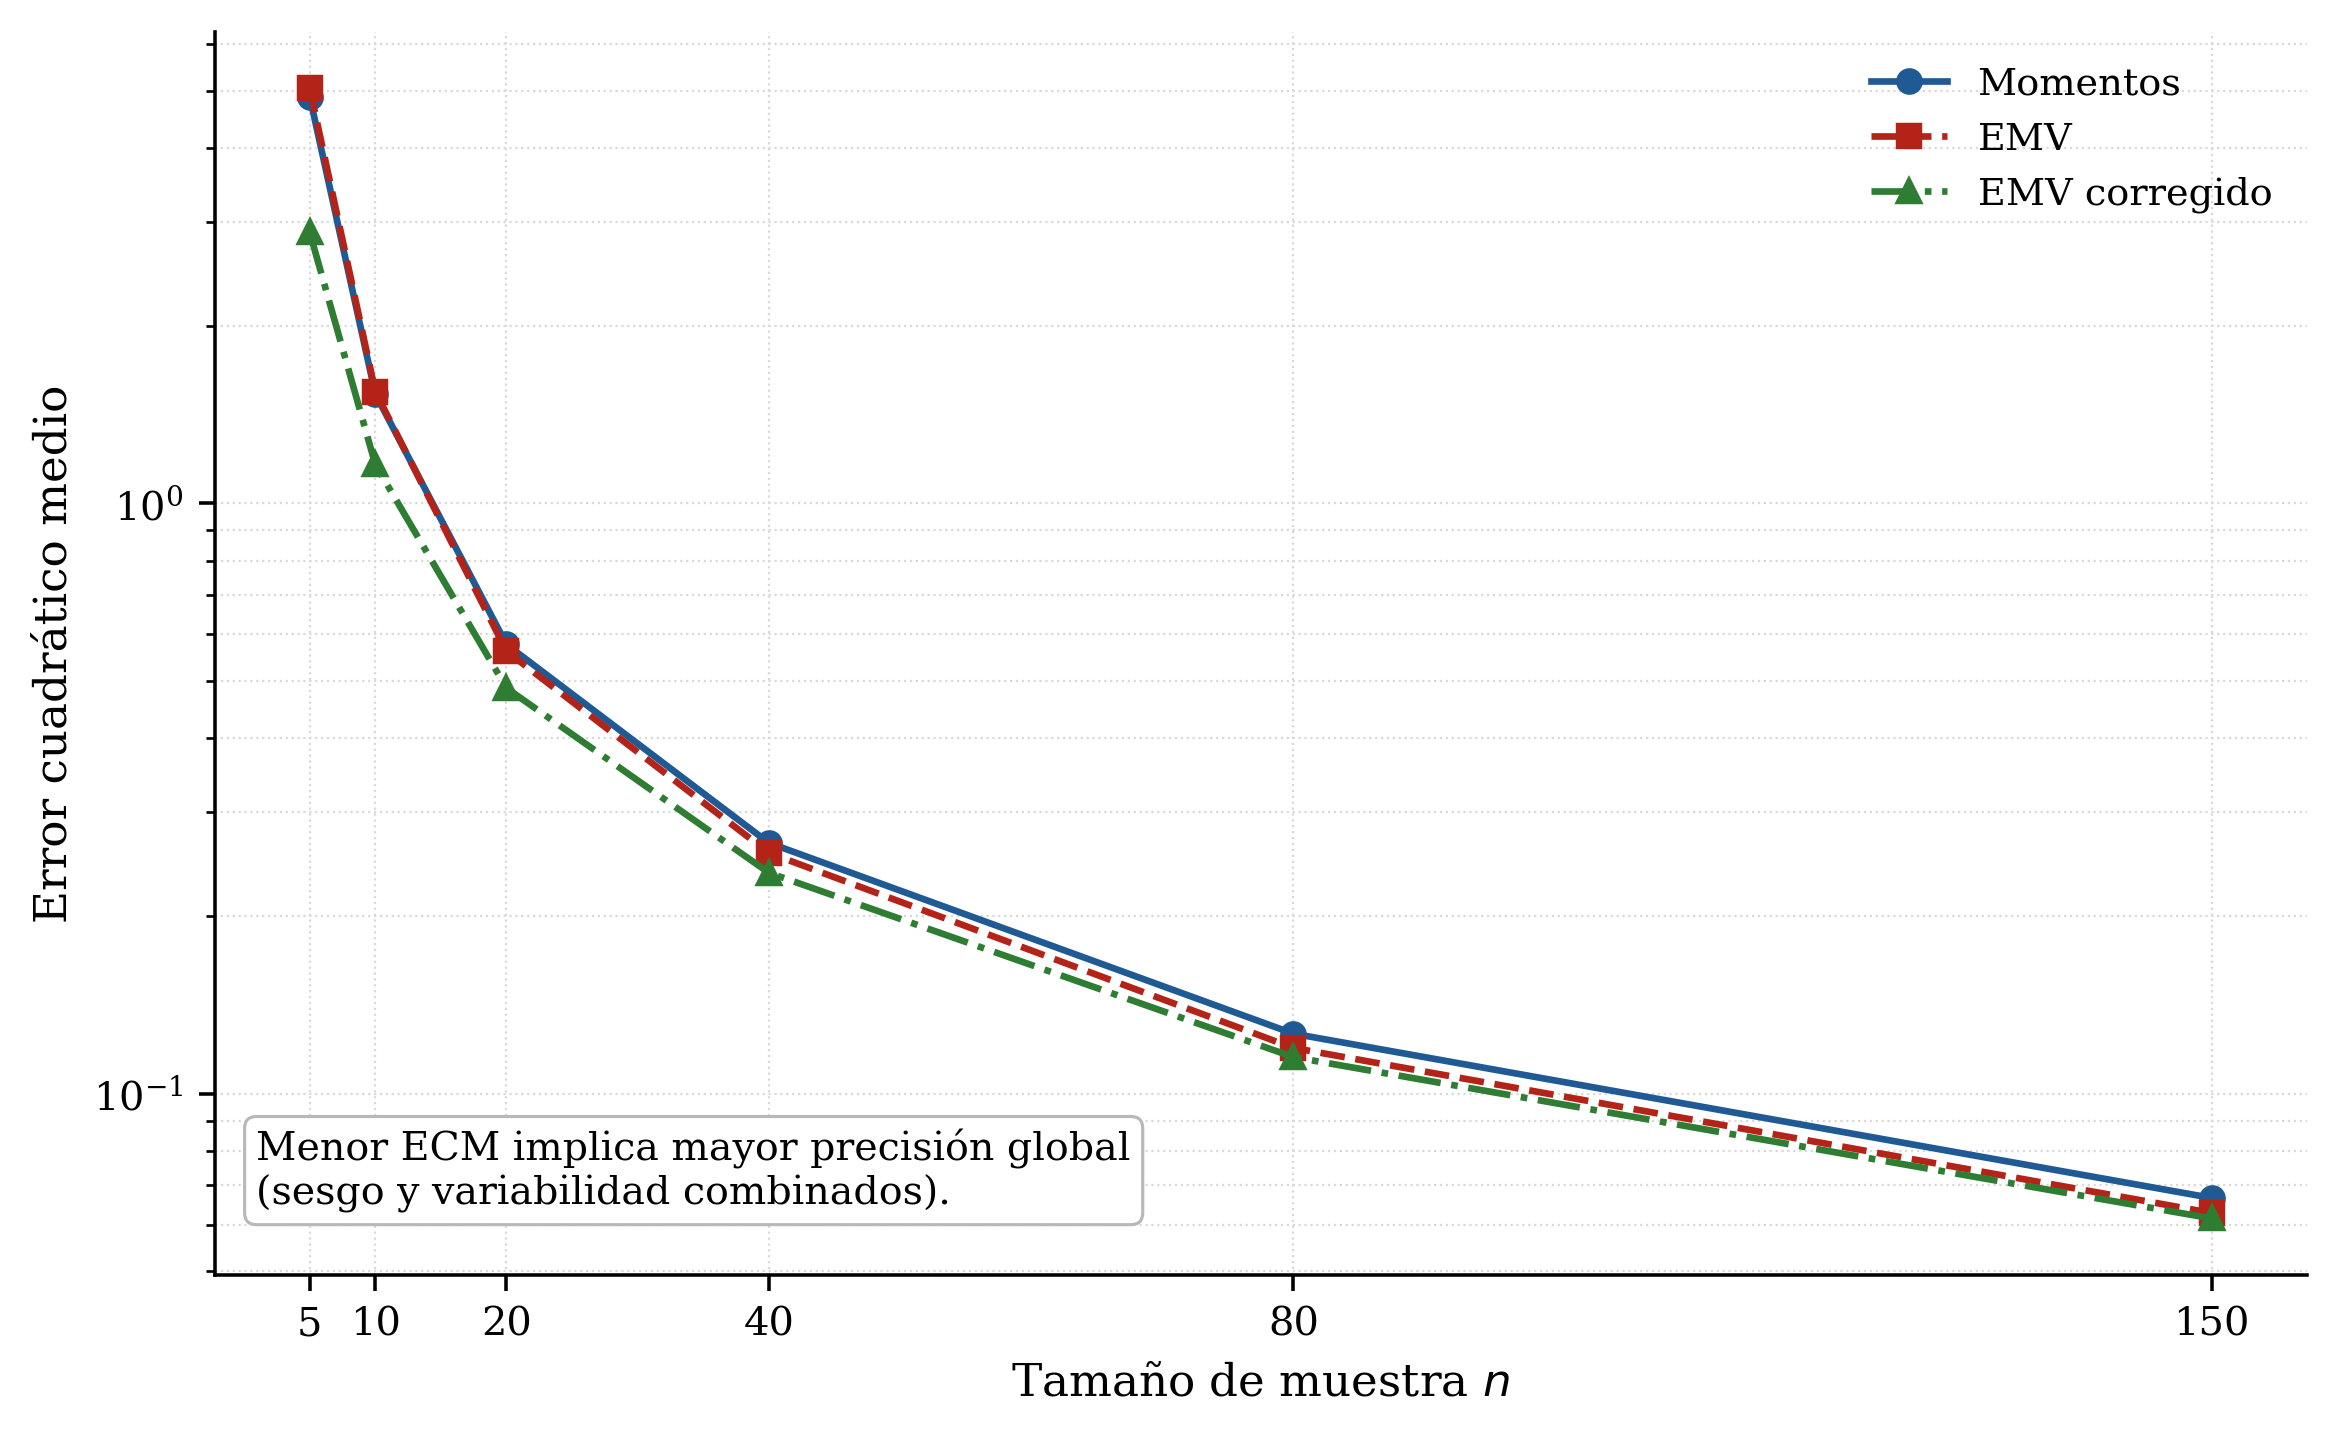
\includegraphics[width=0.91\linewidth]{figures_clear/problema4_estimadores.png}
\caption{Error cuadrático medio de los estimadores de momentos, máxima verosimilitud y estimador de máxima verosimilitud corregido.}
\label{fig:p4}
\end{figure}
\FloatBarrier

\subsection*{Interpretación Figura 5}

El eje horizontal muestra el tamaño de muestra y el eje vertical el ECM estimado mediante las 25\,000 réplicas. Se usa escala logarítmica en el eje vertical para que puedan distinguirse valores que cambian en varios órdenes de magnitud. Una curva más baja significa que, en promedio, el estimador queda más cerca del parámetro verdadero $\theta=2$.

Las tres curvas descienden al aumentar $n$. Esto es la manifestación numérica de la consistencia: con más observaciones, los estimadores fluctúan menos y sus errores cuadrados disminuyen. Para muestras pequeñas, el EMV corregido presenta el menor ECM porque elimina el sesgo positivo del EMV original sin incrementar demasiado su varianza. El estimador de momentos puede producir errores grandes cuando $\overline X$ queda cerca de uno, ya que el denominador $1-\overline X$ se hace pequeño; esas pocas estimaciones extremas elevan el promedio de los errores cuadrados.

A medida que $n$ aumenta, el sesgo del EMV original, $(\theta+1)/(n-1)$, se vuelve pequeño y su curva se acerca a la del estimador corregido. La comparación teórica de varianzas asintóticas predice que el EMV debe superar al método de momentos para muestras grandes. La figura es coherente con esa conclusión, pero además muestra un aspecto que la teoría asintótica no describe por completo: en muestras pequeñas, corregir el sesgo puede ser más importante que la ventaja asintótica de varianza.

\section{Problema 5}

\paragraph{Descripción del problema.}
Se busca construir un intervalo de confianza exacto para $\theta$ en un modelo cuyo soporte depende del parámetro. También se estudia el bootstrap paramétrico y se compara su desempeño con el intervalo exacto mediante simulación.

\subsection*{Elección del estadístico y construcción del intervalo exacto}

La densidad es
\begin{equation*}
f(x;\theta)=\frac{\theta}{x^2},
\qquad x\geq\theta,
\qquad\theta>0.
\end{equation*}
Aquí el soporte depende de $\theta$: todas las observaciones deben ser mayores o iguales que el parámetro. Por esa razón, el mínimo muestral
\begin{equation*}
M=X_{(1)}=\min(X_1,\ldots,X_n)
\end{equation*}
es especialmente informativo y siempre cumple $M\geq\theta$.

Primero se calcula la función de distribución. Para $x\geq\theta$,
\begin{equation*}
F_X(x)=\int_{\theta}^{x}\frac{\theta}{t^2}\,dt
=1-\frac{\theta}{x}.
\end{equation*}
Ahora se busca una transformación sin parámetros. Sea
\begin{equation*}
U_i=\frac{\theta}{X_i}.
\end{equation*}
Para $0<u<1$,
\begin{align*}
P(U_i\leq u)
&=P\!\left(\frac{\theta}{X_i}\leq u\right)\\
&=P\!\left(X_i\geq\frac{\theta}{u}\right)\\
&=1-F_X(\theta/u)=u.
\end{align*}
Por tanto, $U_i\sim U(0,1)$. Como el menor $X_i$ corresponde al mayor cociente $\theta/X_i$,
\begin{equation*}
\frac{\theta}{M}=\max(U_1,\ldots,U_n).
\end{equation*}
Si $V=\max(U_1,\ldots,U_n)$, entonces para $0<v<1$,
\begin{equation*}
P(V\leq v)=P(U_1\leq v,\ldots,U_n\leq v)=v^n.
\end{equation*}
Esta es la función de distribución de una $\operatorname{Beta}(n,1)$, cuyo cuantil $p$ es $p^{1/n}$. Por consiguiente,
\begin{equation*}
P\!\left(
(\alpha/2)^{1/n}\leq\frac{\theta}{M}
\leq(1-\alpha/2)^{1/n}
\right)=1-\alpha.
\end{equation*}
Multiplicando por $M>0$ se obtiene
\begin{equation}
\boxed{
IC_{1-\alpha}(\theta)=
\left[
M(\alpha/2)^{1/n},
M(1-\alpha/2)^{1/n}
\right].}
\label{eq:ic-pareto}
\end{equation}

La verosimilitud ayuda a entender por qué aparece el mínimo:
\begin{equation*}
L(\theta)
=\theta^n\left(\prod_{i=1}^{n}X_i^{-2}\right)
\ind\{0<\theta\leq M\}.
\end{equation*}
Dentro del intervalo permitido $(0,M]$, la parte $\theta^n$ es creciente, así que el máximo ocurre en $\widehat\theta_{EMV}=M$. Además, $\E[M]=n\theta/(n-1)$ para $n>1$, de modo que $(n-1)M/n$ corrige su sesgo. La condición $n>1$ es necesaria porque la esperanza de $M$ solo es finita en ese caso; para $n=1$ no puede justificarse esta corrección mediante insesgamiento. Todas las comparaciones numéricas de este punto se realizan con $n>1$.

\subsection*{Qué significa hacer bootstrap paramétrico}

El bootstrap paramétrico parte de la idea de que, si el modelo es correcto pero $\theta$ es desconocido, se puede sustituir por una estimación y generar nuevas muestras desde el modelo ajustado. En este caso el procedimiento básico es:
\begin{enumerate}
\item calcular $M$ en la muestra original y tomar $\widehat\theta=M$;
\item generar una muestra bootstrap $X_1^*,\ldots,X_n^*$ con densidad $f(x;M)$;
\item calcular $M^*=\min(X_1^*,\ldots,X_n^*)$;
\item repetir muchas veces y usar la distribución de $M^*$ para construir un intervalo.
\end{enumerate}
Para generar cada observación puede usarse la transformación inversa. Si $U\sim U(0,1)$, entonces
\begin{equation*}
X^*=\frac{M}{U}
\end{equation*}
tiene la distribución ajustada.

Sea $q_p^*$ el cuantil de orden $p$ de los mínimos bootstrap $M^*$. El intervalo percentil es $[q_{\alpha/2}^*,q_{1-\alpha/2}^*]$. El intervalo bootstrap básico no usa directamente esos cuantiles, sino que refleja los errores bootstrap $M^*-M$ alrededor del estimador observado. Su forma es
\begin{equation*}
\boxed{
I_{\text{básico}}=
\left[2M-q_{1-\alpha/2}^*,\;2M-q_{\alpha/2}^*\right].}
\end{equation*}
Este intervalo invierte la dirección de los cuantiles respecto a $M$. No obstante, esa corrección no garantiza por sí sola una cobertura exacta, especialmente en un modelo no regular como este; por ello su desempeño debe evaluarse mediante simulación.

El intervalo percentil toma directamente cuantiles de $M^*$. Sin embargo, toda observación bootstrap cumple $X_i^*\geq M$, de modo que
\begin{equation*}
M^*\geq M
\end{equation*}
en todas las réplicas. Los cuantiles percentiles quedan por encima de $M$, mientras que el verdadero parámetro satisface $\theta\leq M$. Por eso este método queda orientado hacia el lado incorrecto y su cobertura es cero en el modelo continuo.

Una alternativa es usar el cociente pivotal
\begin{equation*}
R^*=\frac{M^*}{M}.
\end{equation*}
Su distribución bootstrap imita la de $M/\theta$. Si $r_p^*$ es su cuantil de orden $p$, se invierte la relación para obtener
\begin{equation*}
\boxed{
\left[
\frac{M}{r_{1-\alpha/2}^*},
\frac{M}{r_{\alpha/2}^*}
\right].}
\end{equation*}
Cuando los cuantiles se estiman con muchas réplicas, este intervalo se aproxima al intervalo exacto~\eqref{eq:ic-pareto}.

\subsection*{Procedimiento de simulación}

La comparación de intervalos requiere distinguir dos niveles de repetición. El nivel exterior representa nuevos experimentos realizados bajo el modelo verdadero; el nivel interior representa las muestras bootstrap generadas a partir de cada muestra observada.

En una réplica exterior $r$ se procede así:
\begin{enumerate}
\item se genera una muestra de tamaño $n$ con el valor verdadero fijado de $\theta$; usando la transformada inversa, puede tomarse $X_i=\theta/U_i$ con $U_i\sim U(0,1)$;
\item se calcula el mínimo $M_r$ y se construye el intervalo exacto de~\eqref{eq:ic-pareto};
\item se ajusta el modelo bootstrap usando $\widehat\theta_r=M_r$;
\item se generan $B^*$ muestras bootstrap desde $f(x;M_r)$, se calcula cada mínimo $M_{r,j}^*$ y se obtienen los cuantiles requeridos por los métodos percentil, básico y pivotal;
\item para cada intervalo se registra un indicador igual a uno si contiene al valor verdadero $\theta$ y cero en caso contrario.
\end{enumerate}
Después de $R$ réplicas exteriores, la cobertura empírica del método $m$ es
\begin{equation*}
\widehat C_m=\frac1R\sum_{r=1}^{R}
\ind\{L_{m,r}\leq\theta\leq U_{m,r}\}.
\end{equation*}
También puede calcularse la longitud promedio
\begin{equation*}
\overline{\ell}_m=\frac1R\sum_{r=1}^{R}(U_{m,r}-L_{m,r}),
\end{equation*}
porque una cobertura alta no basta para considerar útil un intervalo si este es excesivamente largo.

En este modelo es posible simplificar el nivel interior. Dado $M_r$, la razón $M_{r,j}^*/M_r$ tiene una distribución que no depende de $M_r$, y puede generarse directamente a partir de uniformes. Esta propiedad reduce el costo computacional sin cambiar el procedimiento estadístico. Aun así, conceptualmente se mantiene la distinción: las réplicas exteriores evalúan la frecuencia de cobertura y las interiores aproximan la distribución bootstrap usada para construir cada intervalo.

La Figura~\ref{fig:p5} usa $\theta=2$, $n=20$, confianza del $95\%$, 40\,000 réplicas exteriores y semilla 1966. En la implementación se aprovecharon los cuantiles conocidos de las razones para evitar un segundo ciclo muy costoso; por eso la variación observada en las barras proviene principalmente del nivel exterior.

\begin{figure}[!htbp]
\centering
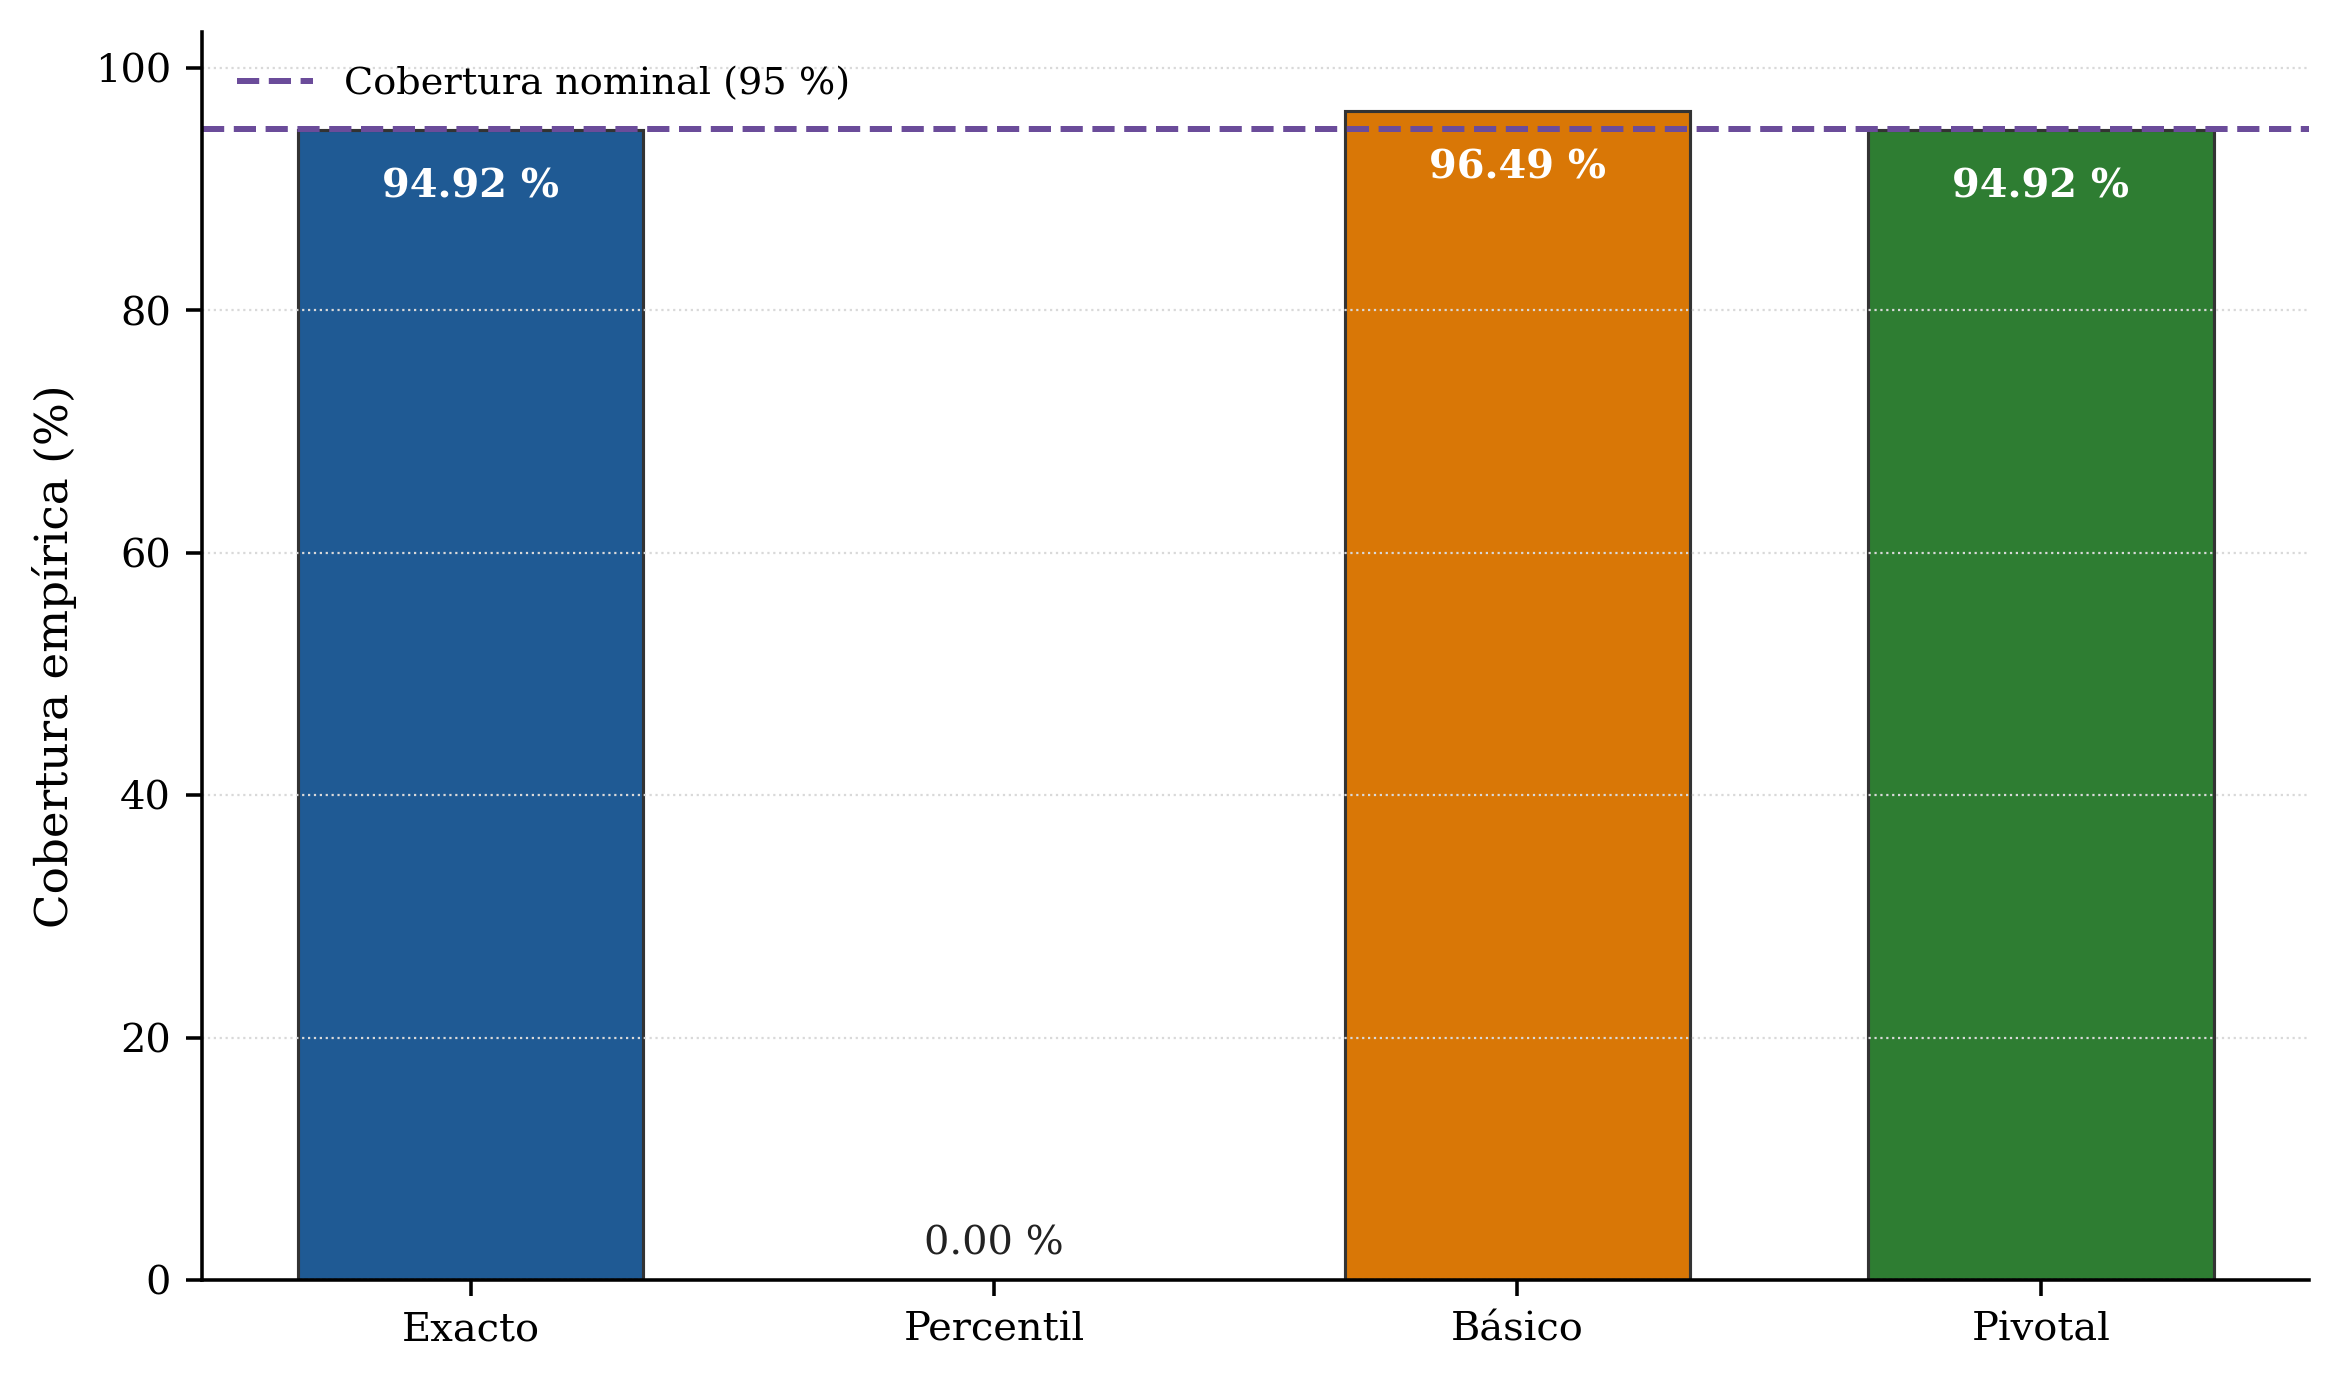
\includegraphics[width=0.89\linewidth]{figures_clear/problema5_bootstrap.png}
\caption{Cobertura empírica de los intervalos exacto, percentil, básico y pivotal.}
\label{fig:p5}
\end{figure}
\FloatBarrier

\subsection*{Interpretación Figura 6}

Cada barra es la proporción de las 40\,000 muestras exteriores en las que el intervalo correspondiente contiene al valor verdadero $\theta=2$. La línea horizontal señala la cobertura nominal del $95\%$. Para los intervalos exacto y pivotal, aproximadamente el $94.92\%$ de los indicadores de cobertura valen uno. La diferencia de $0.08$ puntos porcentuales frente al nivel nominal es pequeña: con $R=40\,000$ y una cobertura cercana a $0.95$, el error Monte Carlo es aproximadamente
\begin{equation*}
\sqrt{\frac{0.95(0.05)}{40\,000}}\approx0.0011,
\end{equation*}
es decir, cerca de $0.11$ puntos porcentuales. Por tanto, el resultado es compatible con la cobertura teórica del $95\%$.

La similitud entre los métodos exacto y pivotal no es casual. Ambos invierten la misma relación de escala entre $M$ y $\theta$; el método exacto usa su distribución conocida y el bootstrap pivotal la reproduce mediante muestras del modelo ajustado.

El intervalo percentil presenta cobertura cero. En cada muestra exterior se cumple $\theta\leq M_r$, mientras que en todas las réplicas interiores $M_{r,j}^*\geq M_r$. Los cuantiles percentiles quedan entonces completamente a la derecha de $M_r$ y no pueden incluir a un parámetro que se encuentra a su izquierda. La falla es estructural y no depende de la semilla ni del número de repeticiones.

El intervalo básico alcanza una cobertura cercana al $96.49\%$ en esta configuración. Su barra superior al $95\%$ indica un comportamiento conservador para estos valores de $n$ y $\theta$, pero no demuestra que funcione igual en todas las configuraciones. La principal conclusión metodológica es que el bootstrap debe adaptarse a la forma del problema. Cuando el soporte depende del parámetro, es necesario revisar la dirección del sesgo y buscar una transformación pivotal antes de aplicar cuantiles de manera automática.

\enlargethispage{2\baselineskip}\section*{A considerar}

El desarrollo muestra que cada procedimiento inferencial debe relacionarse con un fundamento identificable: la distribución de un estadístico, un evento de cobertura, una cota probabilística, la verosimilitud o una cantidad pivotal. Las cantidades calculadas por simulación tampoco se introducen de manera independiente: la cobertura empírica estima una probabilidad de cobertura, el sesgo empírico estima la diferencia entre la esperanza de un estimador y el parámetro, y el ECM empírico estima su error cuadrático promedio. La simulación sirve para verificar, comparar y detectar limitaciones, pero no sustituye las demostraciones analíticas. Todas las figuras usan semilla 1966 para asegurar su reproducibilidad.

\end{document}
